% Assume-se que \textual já foi feito

\newcommand{\multicore}{\textit{multicore}\xspace}
\newcommand{\chip}{\textit{chip}\xspace}
\newcommand{\chips}{\textit{chips}\xspace}
\newcommand{\singlecore}{\textit{single core}\xspace}
\newcommand{\tradeoff}{\textit{trade-off}\xspace}
\newcommand{\exascale}{\textit{Exascale}\xspace}
\newcommand{\greencomputing}{\textit{Green Computing}\xspace}  
\newcommand{\ranking}{\textit{ranking}\xspace}
\newcommand{\bench}{\textit{benchmark}\xspace}
\newcommand{\benchs}{\textit{benchmarks}\xspace}
\newcommand{\capb}{CAP Bench\xspace}
\newcommand{\etal}{\textit{et al}.\xspace}
\newcommand{\thread}{\textit{thread}\xspace}
\newcommand{\threads}{\textit{threads}\xspace}
\newcommand{\cache}{\textit{cache}\xspace}
\newcommand{\caches}{\textit{caches}\xspace}
\newcommand{\byte}{\textit{byte}\xspace}
\newcommand{\bytes}{\textit{bytes}\xspace}
\newcommand{\hardware}{\textit{hardware}\xspace}
\newcommand{\transistor}{\textit{transistor}\xspace}
\newcommand{\transistors}{\textit{transistors}\xspace}
\newcommand{\manycore}{\textit{manycore}\xspace}
\newcommand{\hardware}{\textit{hardware}\xspace}
\newcommand{\mppa}{MPPA-256\xspace}
\newcommand{\cluster}{\textit{cluster}\xspace}
\newcommand{\clusters}{\textit{clusters}\xspace}
\newcommand{\kernel}{\textit{kernel}\xspace}
\newcommand{\kernels}{\textit{kernels}\xspace}
\newcommand{\offset}{\textit{offset}\xspace}
\newcommand{\offsets}{\textit{offsets}\xspace}
\newcommand{\master}{\textit{master}\xspace}
\newcommand{\masters}{\textit{masters}\xspace}
\newcommand{\slave}{\textit{slave}\xspace}
\newcommand{\slaves}{\textit{slaves}\xspace}

\chapter{Introdução}
\label{ch:introdução}

Na última década, a indústria de semicondutores vem investindo largamente na pesquisa e produção de \chips com múltiplos núcleos de processamento em seu interior, chamados de \multicore. Os avanços nessa indústria, juntamente com a área de arquitetura de computadores, são notados desde a década de 1980 em diante, permitindo um crescimento anual em desempenho de 40\% a 50\% \cite{Larus2008} para uma outra classe de processadores nesse período, os de um único núcleo ou \singlecore. Porém, a necessidade de uma nova classe de processadores mostrou-se eminente ao se atingir um ponto onde o \tradeoff entre gasto energético e aumento em desempenho era desproporcional, havendo muita dissipação de calor para pouco crescimento em performance. Essa barreira de potência foi então a responsável pelo interesse da indústria de semicondutores na classe de processadores \multicore. 

Arquiteturas paralelas do tipo \multicore atualmente seguem para uma barreira similar a encontrada pelas \singlecore, visto que, seu principal método de evolução, o aumento no número de núcleos em um mesmo \chip, possui uma limitação, sendo esta o tamanho mínimo que um \transistor pode alcançar, resultando no fim da possibilidade de alocação de mais núcleos em um mesmo espaço, tendo como única opção o aumento do tamanho do \chip. Além disso, soluções que utilizam esse tipo de arquitetura, por exemplo, supercomputadores, estão encontrando o mesmo problema de escalabilidade entre dissipação de calor e ganho em desempenho que os \singlecore encontraram no passado. A Figura \ref{fig:eficienciaxcorestop500} exemplifica esse problema, pois, utilizando a medida de performance \Flops, ou seja, a quantidade de operações de ponto flutuante que um computador realiza por segundo, compara seu crescimento com o aumento no número de núcleos dos supercomputadores com maior poder de computação do mundo ao passar os anos, segundo o \ranking TOP500, mostrando ao mesmo tempo a tendência em aumentar o número de núcleos e a difícil tarefa de encontrar escalabilidade entre esse aumento e o ganho em eficiência.\footnote{Os dados do \ranking TOP500 estão disponíveis no site TOP500: https://www.top500.org/}

Com o interesse atual da comunidade científica em atingir o \exascale e, ao mesmo tempo, em computação voltada para a eficiência energética, pode-se então afirmar que as arquiteturas do tipo \multicore não são mais uma solução viável para os supercomputadores. O alerta do Departamento de Defesa do Governo dos Estados Unidos (DARPA), uma das organizações mais importante do país, serve também como base para essa afirmação, o qual mostrou em um relatório \cite{darpa:exascale} que, para ser viável, um supercomputador que realiza o \exascale deve atingir uma performance de 50 G\Flops/W, enquanto que, atualmente, o supercomputador com o maior poder de processamento do mundo atinge 14.719 G\Flops/W e o de melhor eficiência energética atinge 16.876 G\Flops/W. A Figura \ref{fig:eficienciaxyearstop500} mostra o crescimento na eficiência energética dos supercomputadores mais poderosos do mundo desde 2005\footnote{Foi escolhido este ano como início pois nos anos anteriores a eficiência energética ainda era menor que 0.1 GFlops/W.}, segundo o \ranking TOP500.

\begin{figure}[tb]
  \centering
  \caption{Comparação da evolução da eficiência energética em relação ao número de núcleos do supercomputador número 1 do mundo ao passar dos anos segundo o \ranking TOP500.}
  \label{fig:eficienciaxcorestop500}
  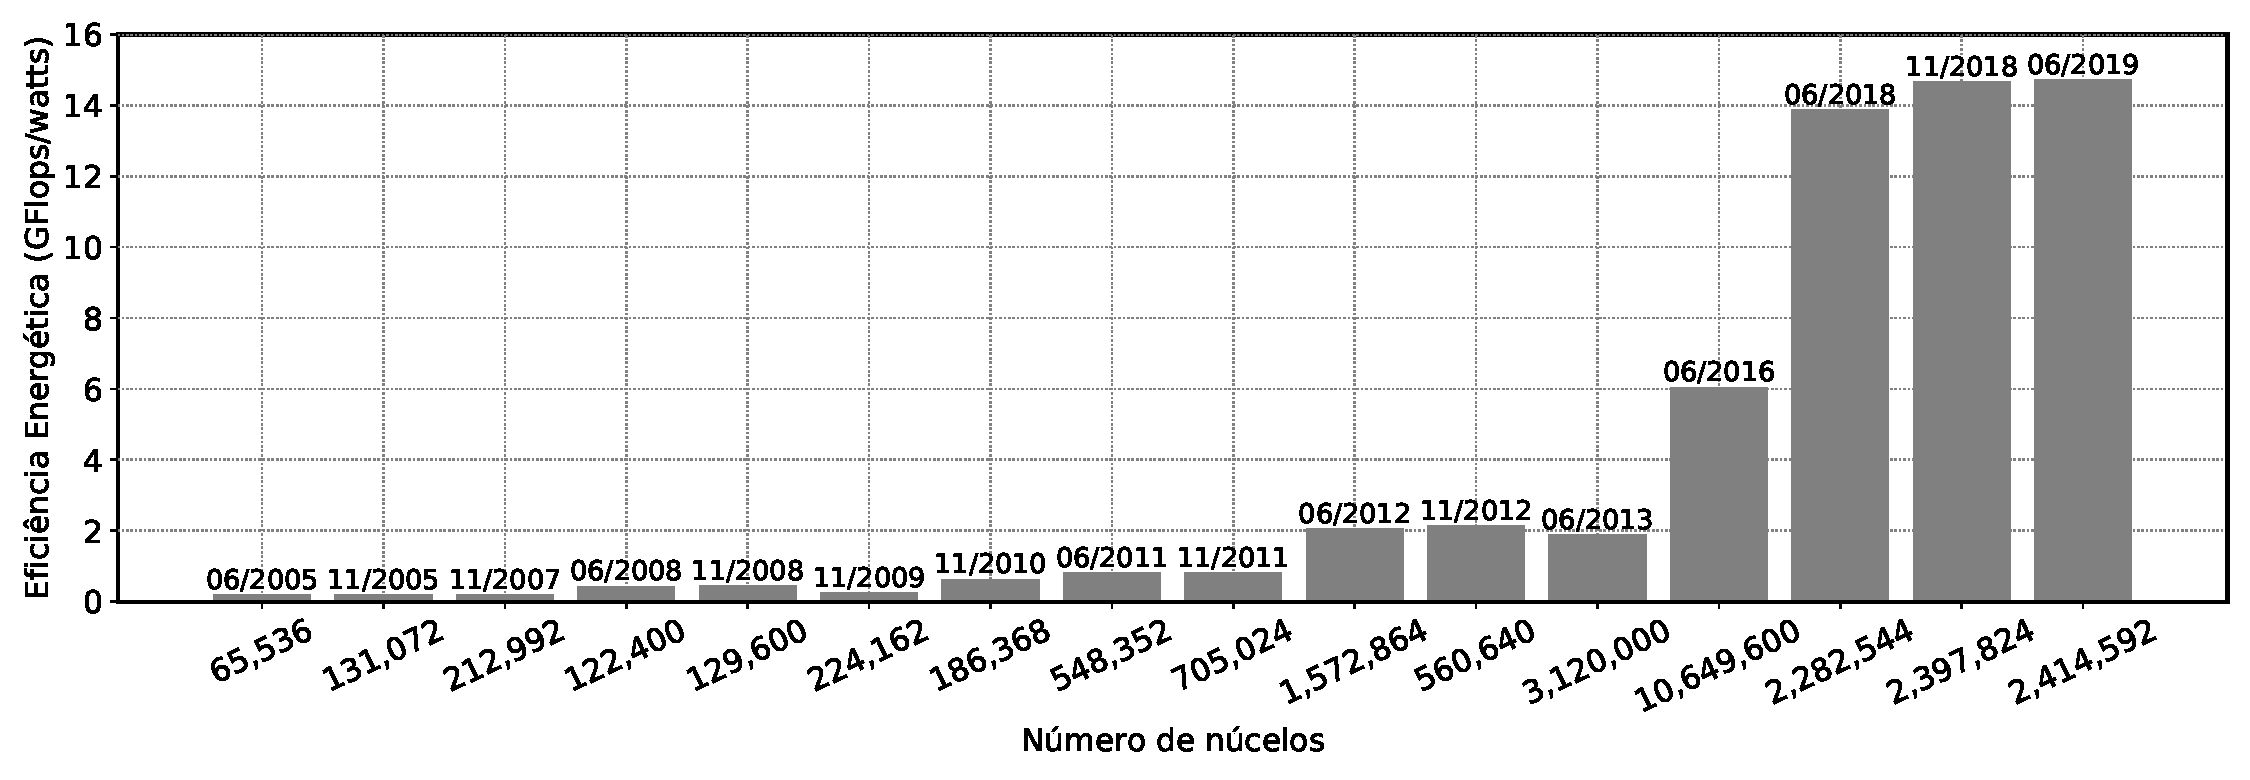
\includegraphics[width=1\linewidth, keepaspectratio]{Figure_Efficiency_X_Cores_Top500.pdf}
  \fonte{Gráfico desenvolvido pelo autor.}
\end{figure}

\begin{figure}[tb]
  \centering
  \caption{Evolução da eficiência energética do supercomputador número 1 do mundo segundo o \ranking TOP500.}
  \label{fig:eficienciaxyearstop500}
  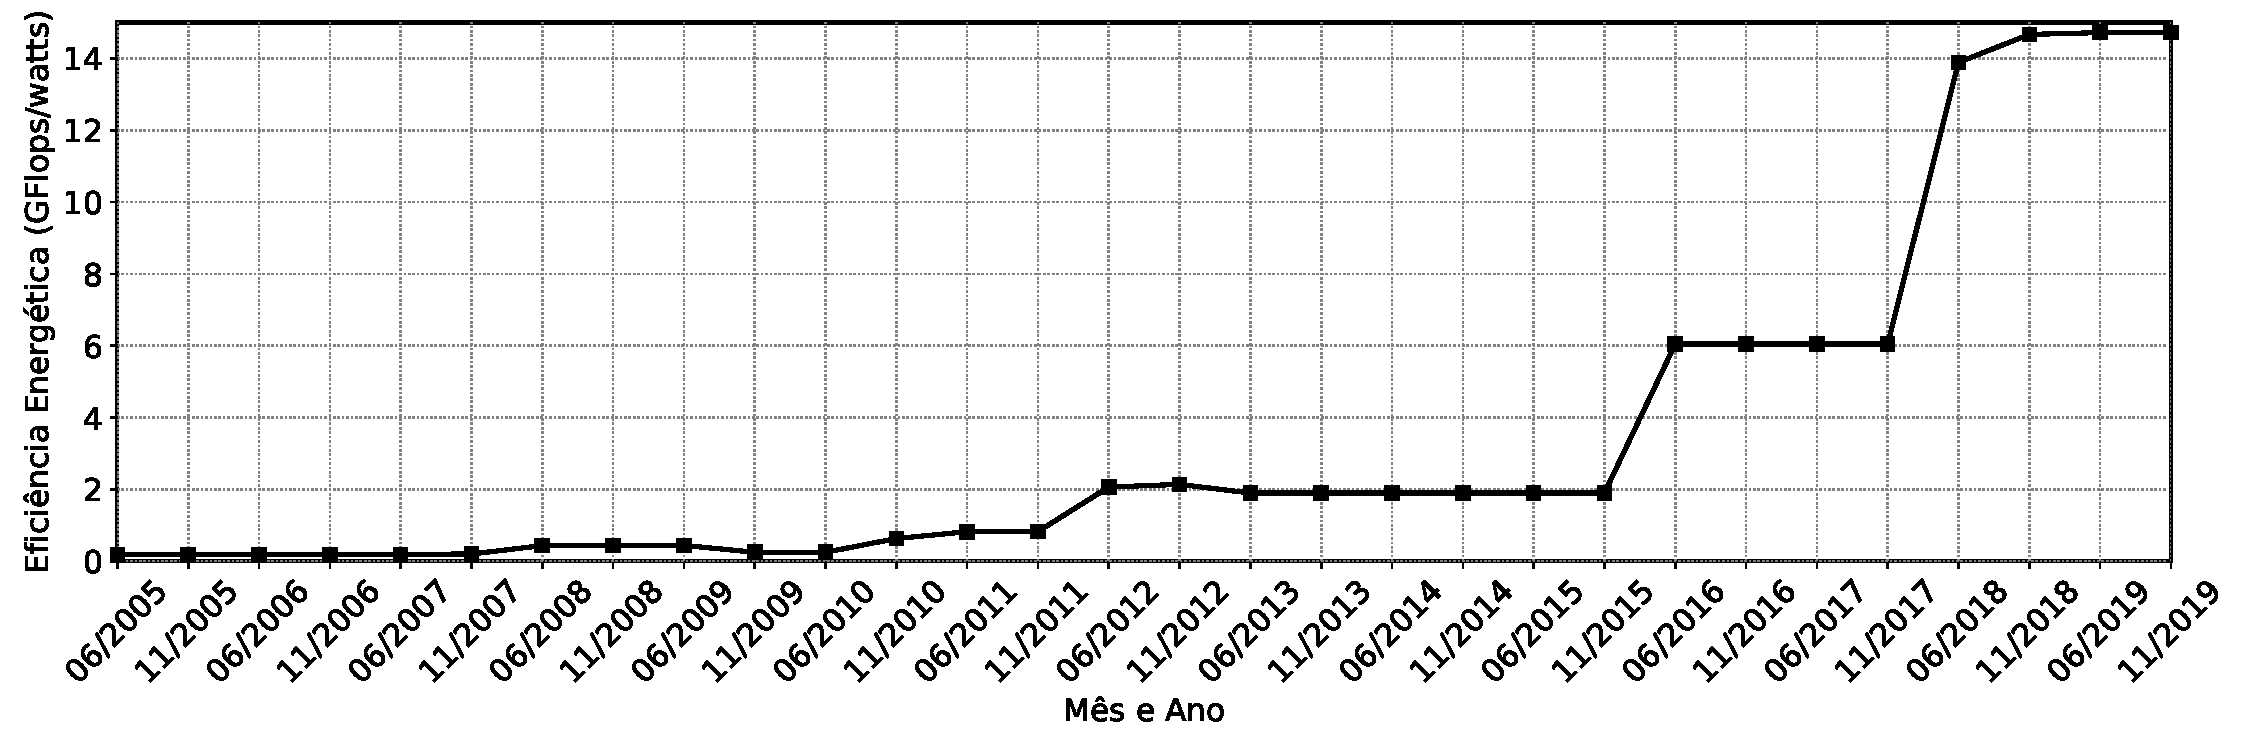
\includegraphics[width=1\linewidth, keepaspectratio]{Figure_Efficiency_X_Years_Top500.pdf}
  \fonte{Gráfico desenvolvido pelo autor.}
\end{figure}

Buscando novos tipos de arquiteturas paralelas que apresentem as características faltantes no problema de balanceamento apresentado acima, pesquisadores da área de \HPC realizaram diversos estudos voltados para essa questão, aplicando conceitos de \greencomputing \cite{greencomputingacm} no decorrer do desenvolvimento de suas soluções. Dentre estas soluções, temos o surgimento da classe de processadores \manycore de baixa potência, como o \mppa \cite{mppa2562013}, objeto de estudo deste trabalho, o Adapteva Epiphany \cite{olofsson2014}, e o SW26010, utilizado no atual terceiro supercomputador mais poderoso do mundo, o \textit{Sunway TaihuLight} \cite{fu2016sunway}. Vale citar que o SW26010 desbancou em 2016 o supercomputador que assumia, desde 2013, a primeira posição do \ranking TOP500, obtendo duas vezes mais desempenho que esse e reduzindo em três vezes o consumo energético, explicando também o ganho elevado em eficiência em ambas as Figuras \ref{fig:eficienciaxcorestop500} e \ref{fig:eficienciaxyearstop500} no mês de junho de 2016.

Para avaliar o desempenho e consumo energético do \mppa, \textit{Souza} \etal \cite{astro-Souza-CCPE:2016} propuseram o desenvolvimento do \bench \capb, o qual, em sua primeira versão, utilizava uma \API de comunicação síncrona entre processos denominada \IPC \cite{mppa2562013}. Essa \API possui algumas deficiências, como o baixo nível de abstração, requerendo conhecimento prévio da arquitetura alvo para implementações paralelas eficientes, e a realização de sincronizações implícitas muitas vezes não necessárias nas operações de envio e recebimento de dados, o que leva a queda de desempenho da aplicação. Ao realizar a otimização do \bench, \textit{David} \etal o portaram com a \ASYNC, uma \API com maior nível de abstração e com conceitos de assincronismo, aumentando o potencial de desempenho da aplicação. Além disso, alterações na implementação de todas as aplicações foram realizadas de modo a otimizá-las ainda mais.

Portanto, para realizar uma comparação justa entre as \APIs citadas acima, faz-se necessário atualizar a lógica de implementação das aplicações da versão antiga do \bench, para que essas se equivalham às novas implementações, criando assim um ambiente propício para comparar aspectos puramente das tecnologias de comunicação citadas, utilizando as duas versões do \bench para isso. A comparação entre ambas as implementações será responsável por determinar qual \API se comporta de maneira mais robusta no \mppa em certos contextos, onde os dados acerca do tempo de execução, quantidade de dados enviados e recebidos e gasto energético de cada aplicação serão as métricas para essa determinação. Assim, teremos dados de execução das duas \APIs numa mesma versão de placa do \mppa, resultando numa base de dados concreta para a tomada de decisão sobre qual das duas \APIs escolher na hora de implementar uma nova aplicação.

\section{Objetivos}
\label{sec:objetivos}

Com base no que foi exposto, são apresentados abaixo o objetivo geral e os objetivos específicos deste trabalho.

\subsection{Objetivo Geral}
\label{sec:objetivogeral}

O objetivo deste trabalho é obter dados concretos acerca da execução de aplicações de diversos domínios de problemas no \mppa, utilizando as duas \APIs já citadas e o \capb, podendo assim comparar as execuções de cada aplicação em cada cenário específico possível dentro do processador, obtendo identificadores precisos que, em momentos futuros, possam apontar qual das duas \APIs utilizar, dependendo do domínio de problema de uma certa aplicação.

\subsection{Objetivos Específicos}
\label{sec:objetivosespecifico}

\begin{itemize}
\item Investigar a viabilidade do uso do \mppa para a área de \HPC.
\item Estudar aspectos das \APIs de comunicação existentes no \mppa, mais especificamente, a \ASYNC e a \IPC.
\item Avaliar os custos e benefícios do \mppa em relação ao desempenho e gasto energético, assim como sua utilidade para a Computação Sustentável (\greencomputing)
\item Comparar as \APIs \ASYNC e \IPC a fim de prover métricas precisas para a escolha de uma das duas numa futura implementação.
\end{itemize}

\section{Contribuições do trabalho}

Este trabalho é continuação de um projeto de iniciação científica desenvolvido por \textit{David} \etal, o qual resultou em um resumo expandido publicado na Escola Regional de Alto Desempenho da Região Sul no ano de 2019:

\begin{itemize}
  \item ORDINE, D. G. V.; PODESTA JUNIOR, E. ; PENNA, P. H. ; CASTRO, M. \textbf{Otimização de Aplicações do CAP Bench para o Processador \mppa.} In: Escola Regional de Alto Desempenho da Região Sul (ERAD/RS), 2019, Três de Maio. Anais da Escola Regional de Alto Desempenho da Região Sul (ERAD/RS). Porto Alegre: Sociedade Brasileira de Computação (SBC), 2019.
\end{itemize}

\section{Organização do trabalho}

Este trabalho está dividido da seguinte forma. O Capítulo \ref{ch:fundamentacaoteorica} mostra os conceitos teóricos que foram utilizados para a produção dessa dissertação. O Capítulo \ref{ch:trabcorrelatos} apresenta alguns trabalhos relacionados a este. O Capítulo \ref{ch:desenvolvimento} contém toda a proposta deste projeto, detalhando tudo que foi feito, assim como explicando as métricas que serão expostas nos resultados. O Capítulo \ref{ch:resultados} apresenta os resultados preliminares já obtidos. Para finalizar, o Capítulo \ref{ch:conclusao} conclui este trabalho.

\chapter{Fundamentação Teórica}
\label{ch:fundamentacaoteorica}

Neste capítulo são apresentados conceitos relacionados a Computação Paralela, por exemplo, padrões arquiteturais, na Seção \ref{sec:arquiteturasparalelas}, e tecnologias de programação, na Seção \ref{sec:bibliotecasdevparalelo}. Também são mostrados algumas características do \mppa na Seção \ref{sec:mppa256}.

\section{Arquiteturas Paralelas}
\label{sec:arquiteturasparalelas}

Existem três tipos de sistemas com múltiplos processadores, segundo \textit{Tanenbaum} \etal : os multiprocessadores, os multicomputadores e os sistemas distribuídos \cite{TanenbaumMordenOS}. São detalhados nesta seção conceitos acerca das arquiteturas multiprocessadores e multicomputadores.

\subsection{Multiprocessadores}
\label{sec:multiprocessadores}

A principal característica de uma arquitetura multiprocessador é o acesso compartilhado ao barramento de memória do sistema, a \RAM, por diversas \CPUs. Programas executando em qualquer um dessas \CPUs possuem espaços de endereçamento físicos únicos na \RAM e as \threads de um desses programas fazem uso de um mesmo espaço de memória, através de operações de escrita e leitura, para se comunicarem. Um fato peculiar dessa arquitetura é a possibilidade de ocorrer problemas de concorrência quando duas ou mais \threads de um mesmo programa executam em diferentes \CPUs, onde, na visão de uma \CPU, ela escreve um valor em uma posição de memória e lê outro valor daquela mesma posição, pois uma \thread executando em outra \CPU alterou o valor daquela posição. 

Multiprocessadores são também classificados em dois tipos, de acordo com a velocidade de acesso a uma posição de memória. Quando uma certa palavra na memória pode ser lida na mesma velocidade que qualquer outra, são chamados de multiprocessadores com acesso uniforme a memória - \UMA. Já quando a velocidade de leitura em diferentes posições de memória muda, são chamados de multiprocessadores com acesso não uniforme a memória - \NUMA. 

A arquitetura mais simples de um multiprocessador \UMA, exemplificada na Figura \ref{fig:umasimples}, envolve um único barramento conectando duas ou mais \CPUs a um módulo de memória, permitindo que todas as \CPUs realizem operações de leitura e escrita neste módulo. Quando uma \CPU necessita ler alguma palavra da memória, primeiramente ela verifica se o barramento está ocupado. Caso não, informa à memória, através do barramento, qual endereço deseja obter o valor, aguardando o recebimento deste pelo mesmo barramento. Caso esteja, a \CPU aguarda a liberação do barramento. Para uma pequena quantidade de \CPUs, o tempo de espera médio para o acesso ao barramento tende a ser pequeno e tolerável. Porém, quando elevam-se em algumas dezenas o número de \CPUs observa-se o principal problema deste exemplo de arquitetura \UMA: a ociosidade, por muito tempo, de grande parte das \CPUs, enquanto aguardam pelo acesso ao barramento.



\begin{figure}[tb]
  \centering
  \caption{Diferentes esquemas possiveis de um multiprocessador UMA baseado em barramento.}
  \subcaptionminipage[fig:umasimples]%
    {.4\linewidth}%
    {Sem \textit{cache}}%
    {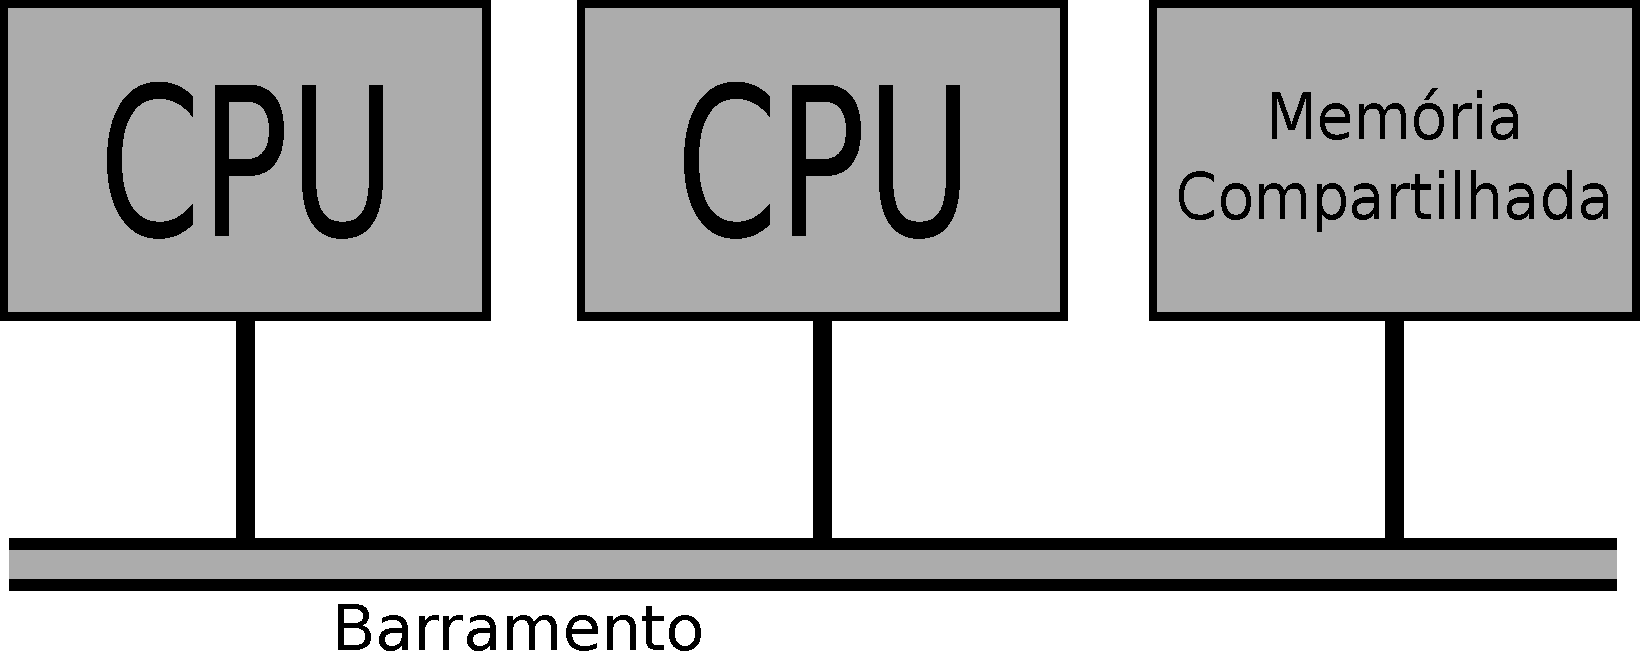
\includegraphics[width=.9\linewidth]{umasimples.pdf}}%
  \hfill% 
  \subcaptionminipage[fig:umacomcache]%
    {.4\linewidth}%
    {Com \textit{cache}}%
    {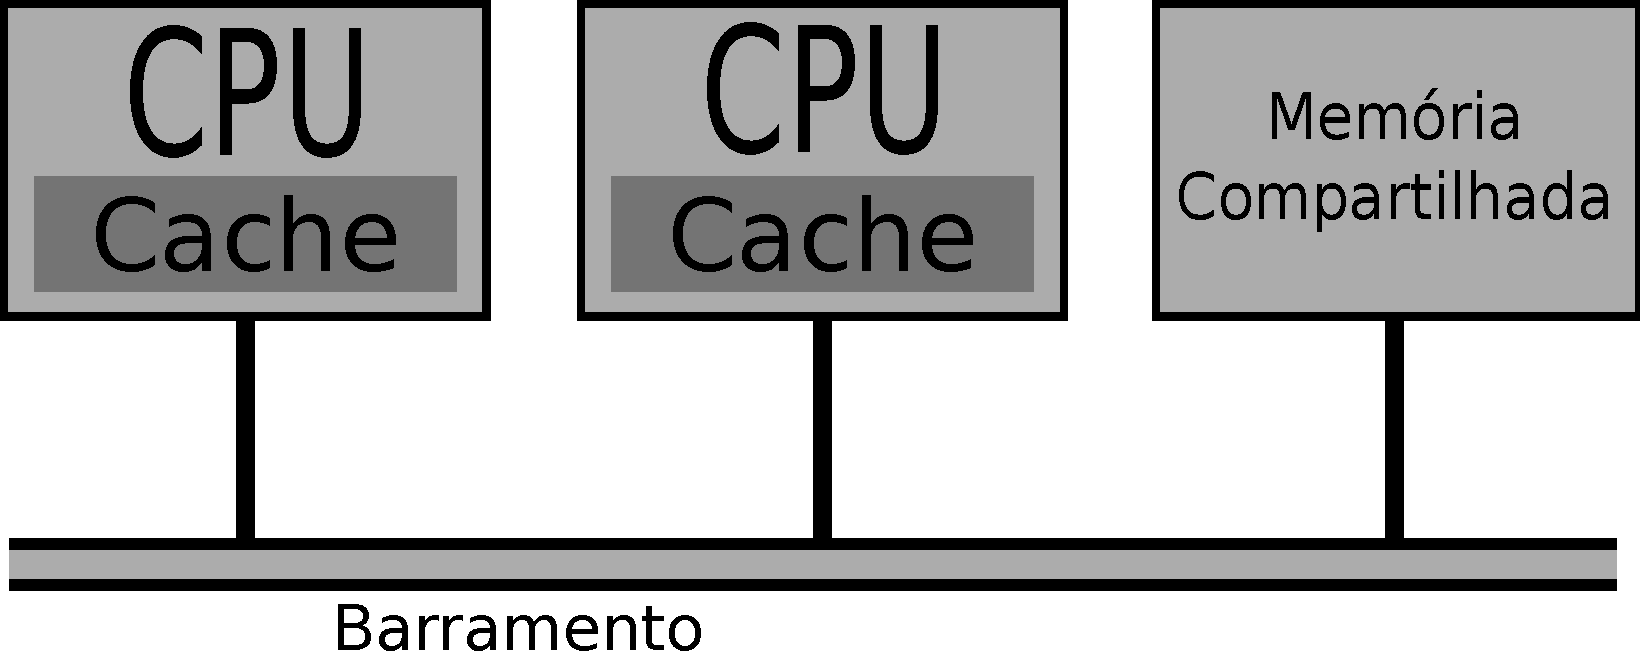
\includegraphics[width=.9\linewidth]{umacomcache.pdf}}%
  \hfill% 
  \subcaptionminipage[fig:umacomcacheememprivada]%
    {.4\linewidth}%
    {Com \textit{cache} e memórias privadas}%
    {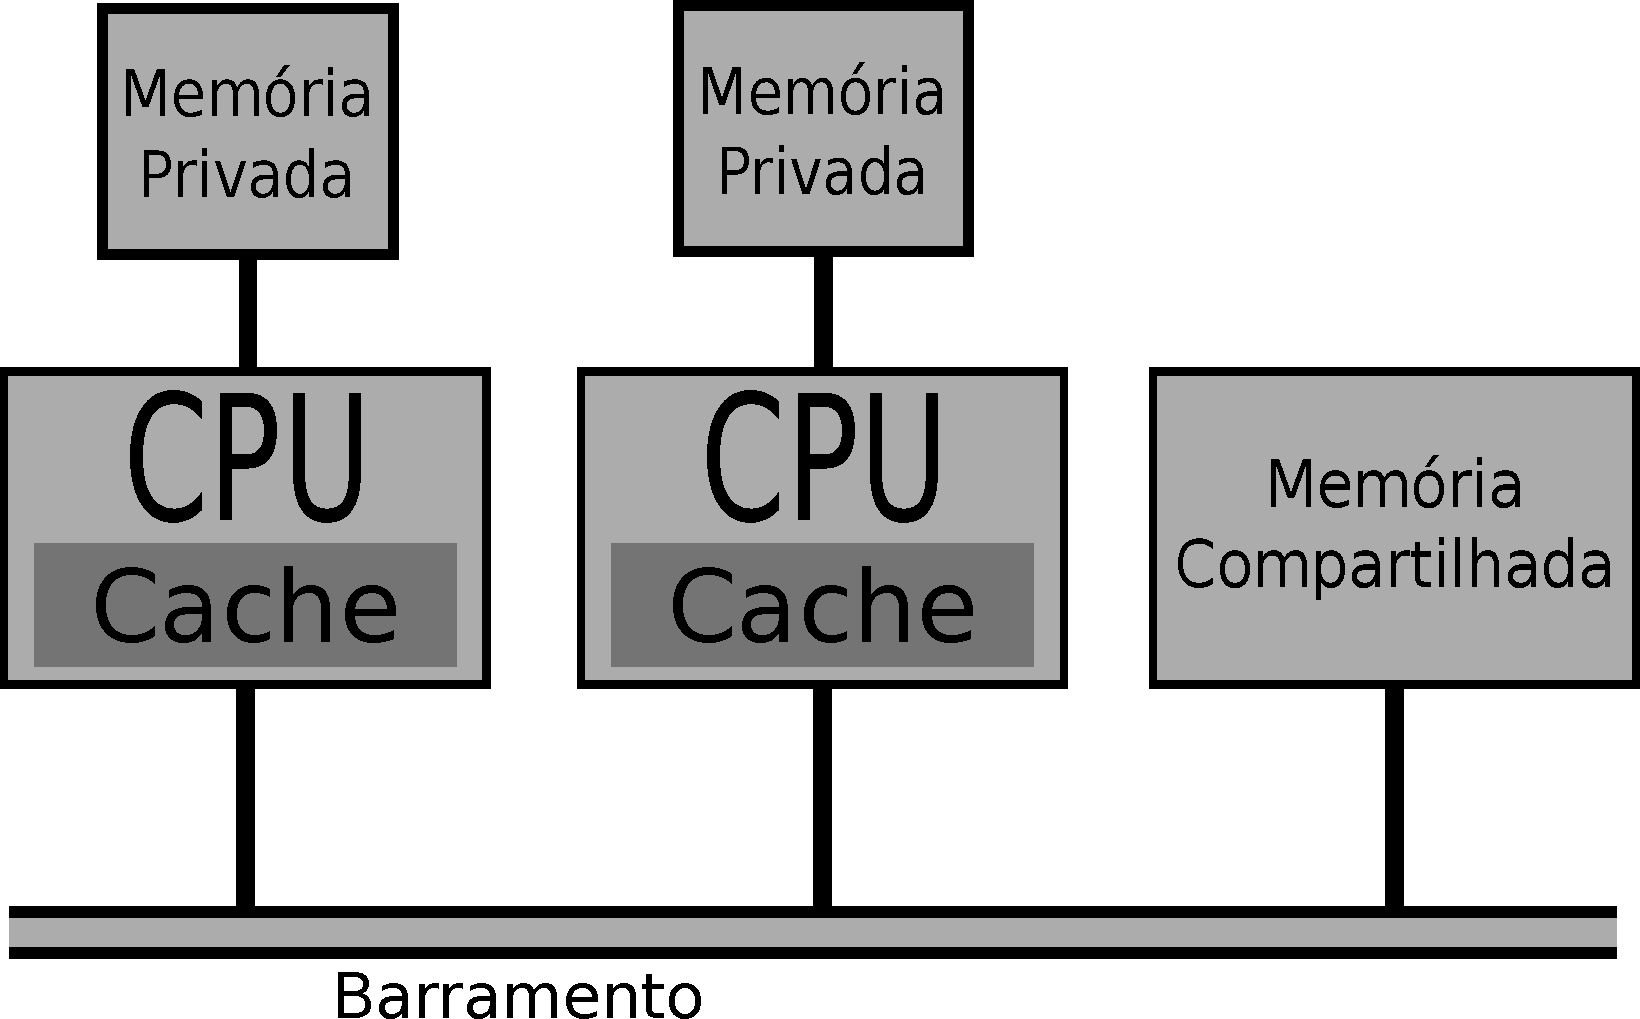
\includegraphics[width=.9\linewidth]{umacomcacheememprivada.pdf}}%
  \hfill% 
  \fonte{Imagens desenvolvidas pelo autor, adaptadas de \textit{Tanenbaum} \etal \cite{TanenbaumMordenOS}.}
\end{figure}

Adicionar \caches às \CPUs, como na Figura \ref{fig:umacomcache}, é uma solução para reduzir o gargalo imposto sobre o barramento, já que agora valores podem ser lidos diretamente da \cache local, a qual está muito mais próxima da \CPU e possui tempo de acesso muito menor. Outra possibilidade é adicionar, além das \caches, memórias privadas locais,  como na Figura \ref{fig:umacomcacheememprivada}. Compiladores podem colocar nessas memórias todos os dados que são somente de leitura, por exemplo, constantes, o código do programa, strings e pilhas, utilizando assim esta segunda configuração de forma otimizada. Ambas configurações removem grande parte do tráfego no barramento, tornando seu uso exclusivamente para as variáveis compartilhadas entre \threads.

A adição de \caches impõe uso de protocolos de coerência para que não haja inconsistência entre os valores de um mesmo endereço de memória nas diferentes \caches. Primeiramente, para otimizar as operações de leitura, quando uma palavra é referenciada, todo o bloco que contém essa palavra, geralmente de 32 ou 64 \bytes, é colocado na \cache. Já para garantir a coerência, cada bloco é marcado como sendo somente de leitura, podendo assim estar presente em outras \caches, ou de leitura e escrita, não devendo estar presente em nenhuma outra \cache neste caso. Quando uma \CPU tenta alterar um valor que está presente em outras \caches além de sua própria, o \hardware do barramento informa essa operação às outras \caches, as quais tratam esse contexto de duas formas. Caso o valor da \cache seja o mesmo em memória, podem simplesmente descartá-lo, buscando o novo valor na memória se necessário. Caso outra \cache tenha um valor diferente daquele em memória, é necessário ou salvá-lo na memória ou transferi-lo diretamente para a \cache que solicitou a operação de escrita.

Quando necessita-se de um número de processadores na ordem das centenas, a arquitetura \UMA acaba sendo inviável. Assim, introduz-se a arquitetura \NUMA, trazendo com ela a ideia de diferentes tempos de acesso para diferentes posições de memória. Multiprocessadores \NUMA provém essa escalabilidade implementando um espaço de endereçamento único para todas as \CPUs através de uma rede de interconexão, como na Figura \ref{fig:multiprocessadornuma}, o que causa a diferença nos tempos de acesso, os quais serão totalmente dependentes do local da memória que se deseja acessar um valor relativo ao local da \CPU que requisitou este acesso. Logo, outra propriedade desta arquitetura é o acesso mais rápido à memória local de um ou um conjunto de \CPUs, em comparação com o acesso à memória remota. Vale salientar que programas desenvolvidos para multiprocessadores \UMA conseguem ser executados em arquiteturas \NUMA, devido a ambas possuírem um espaço de endereçamento único. Porém, estes programas irão obter performance inferior, já que não foram otimizados para considerar as diferenças de tempo entre acesso à memória local e remota.

\begin{figure}[tb]
  \centering
  \caption{Esquema genérico de um multiprocessador NUMA.}
  \label{fig:multiprocessadornuma}
  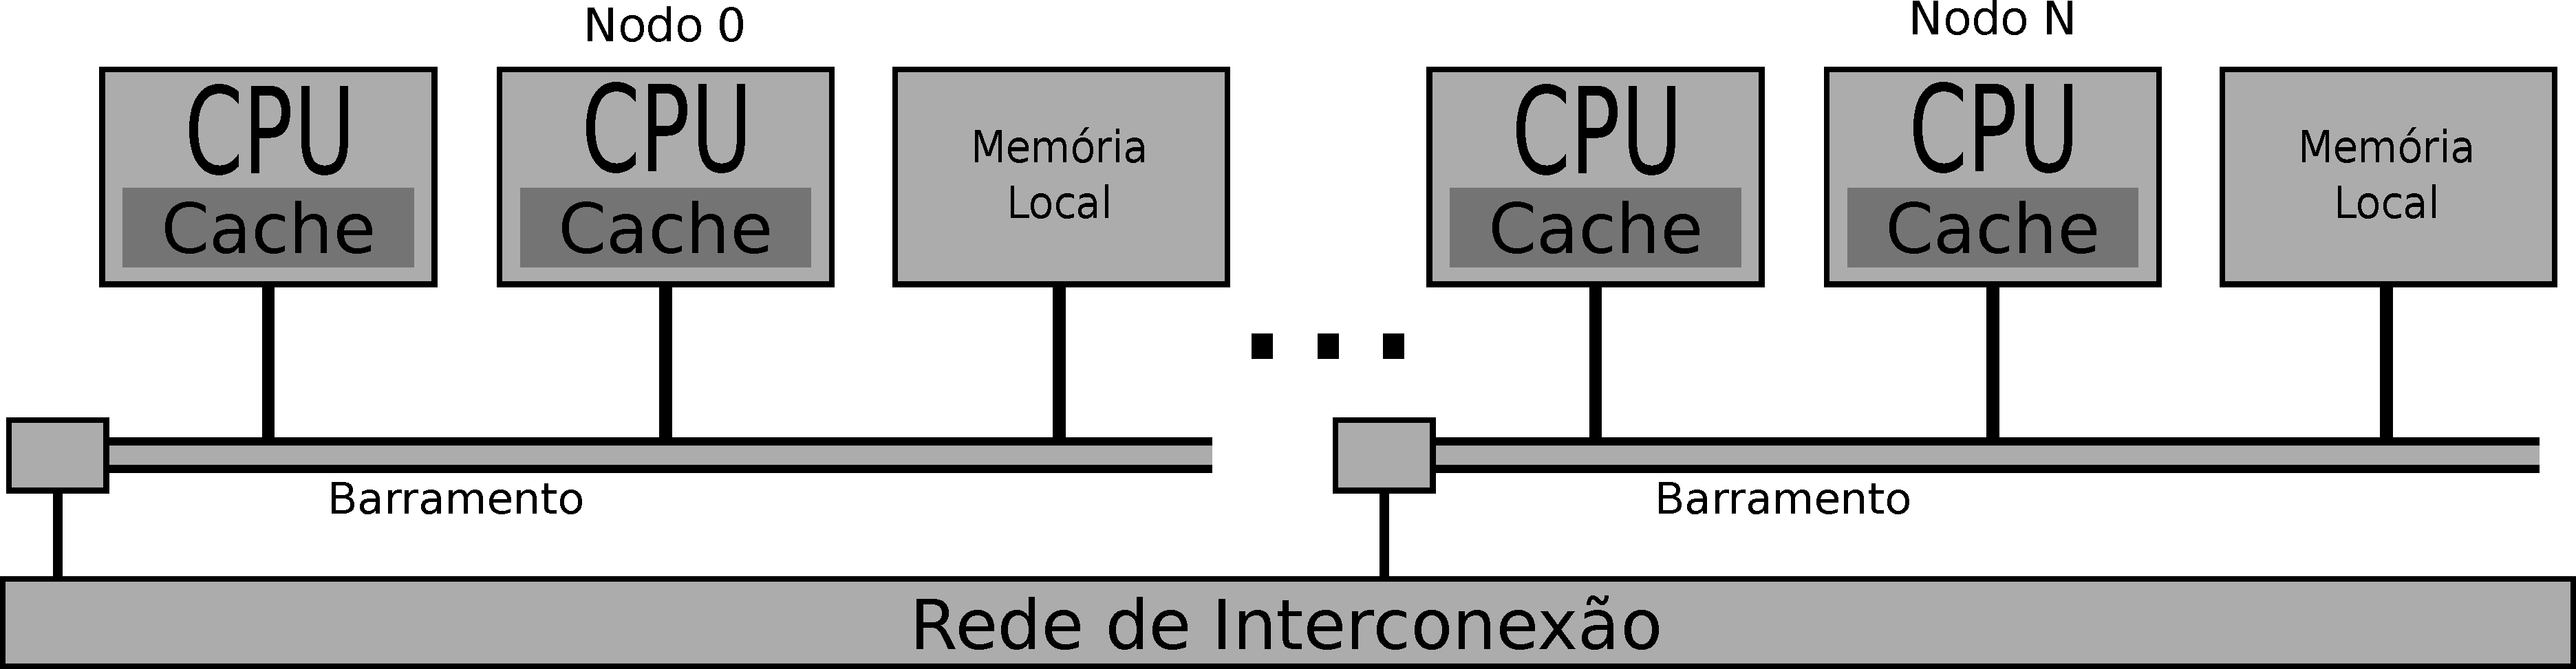
\includegraphics[width=.9\linewidth, keepaspectratio]{numa.pdf}
  \fonte{Imagem desenvolvida pelo autor, adaptada de \textit{Tanenbaum} \etal \cite{TanenbaumMordenOS}.}
\end{figure}

A medida que o tamanho de um \transistor diminui, o número de \transistors em um \chip tende a aumentar. Diversas soluções exploram o que fazer com este número crescente de \transistors, por exemplo, adicionar \caches poderosas de muitos \textit{mega}\bytes ou colocar duas ou mais \CPUs, também chamadas de núcleos (em inglês \textit{cores}), neste mesmo \chip. Em certo ponto, o aumento no tamanho da \cache traz pouquíssimo ganho em porcentagem de \textit{hit} (quantidade de vezes que é possível buscar um dado diretamente na \cache), mostrando assim que o investimento no paralelismo trazido pelos múltiplos núcleos como recurso para ganho em desempenho é uma opção a se considerar. Assim, \chips \multicore são uma mescla de múltiplas \CPUs com múltiplos níveis de \cache inseridos em um espaço muito menor que um multiprocessador, sendo por isso também chamados de \CMPs.

Apesar de serem parecidos, existem algumas diferenças entre os \CMPs e os multiprocessadores. Primeiramente, em muitos \CMPs ocorre o compartilhamento da \cache nível 2 ou 3 entre suas \CPUs, o que não acontece nos multiprocessadores, que possuem \caches totalmente privadas em todos os níveis. Além disso, a probabilidade de que falhas em componentes compartilhados levem a impossibilidades em múltiplas \CPUs ao mesmo tempo é muito maior nos \CMPs, devido a proximidade de conexão das \CPUs. Por fim, existem \chips \multicore em que todos os núcleos são feitos para atender a uma ampla gama de contextos, enquanto que em outros, além das \CPUs principais, existem também núcleos específicos para alguns problemas, como decodificação de áudio e vídeo ou interfaces de rede. 

Apesar de não haver uma barreira de distinção entre um \chip \manycore ou \multicore, pode-se chama-lo de \manycore quando a perda de um núcleo tem um pequeno impacto na performance total do \chip. Um problema com arquiteturas \manycore é a escalabilidade entre manter as \caches de todas as \CPUs coerentes e ainda assim elevar o desempenho ao elevar o número de núcleos. Cientistas da área de \HPC temem que essas duas variaveis não escalem proporcionalmente, tornando o custo de gerenciar essas \caches tão alto que a adição de um novo núcleo de pouco ajudara no aumento em performance. Este problema é também conhecido como a barreira de coerencia  (\textit{coherency wall}) \cite{TanenbaumMordenOS}.

Para o futuro dos \manycore, espera-se processadores que invistam mais  na comunicação entre \CPUs através da troca de mensagens extremamente rápidas via \hardware e através de uma memória compartilhada, deixando de lado parte da coerência de \cache. Uma \GPU é um dos exemplos mais comuns de um processador \manycore, possuindo milhares de pequenos núcleos especializados na rápida execução de cálculos e sem uma lógica complexa de \cache, ou seja, priorizam o processamento. Desta maneira, \GPUs são excepcionais para a execução paralela de pequenas tarefas, como a renderização de \textit{frames} para jogos. Programar para uma \GPU é uma tarefa difícil e muitas vezes algumas linguagens de programação especiais são utilizadas, como a OpenGL ou a CUDA, da NVIDIA. Essa dificuldade se dá, principalmente, pelo fato dos núcleos de uma \GPU executarem exatamente a mesma instrução em diferentes fatias de um dado, ou seja, pelo fato da \GPU ser uma máquina \SIMD.

\subsection{Multicomputadores}
\label{sec:multicomputadores}

Multicomputadores surgiram na dificuldade de aumentar o poder de processamento de um multiprocessador quando se atinge grandes escalas em relação ao número de núcleos. Ao contrário dos multiprocessadores, multicomputadores não compartilham memória, sendo relativamente fáceis de se construir, tendo como componente principal um computador com uma placa de rede de alta performance, sem mouse, teclado e monitor. Neste sistema, também chamado de \textit{Cluster Computers} ou {Cluster Of Workstations} (COWs), é necessário um \textit{design} inteligente da rede que irá conectar os computadores para que se possa obter um alto desempenho.

Um nó de um multicomputador consiste então em um computador, com uma \CPU, memória, placa de rede e um HD. Diversas são as topologias possíveis para a rede que conecta os nós, como mostrado na Figura \ref{fig:topologiamulticomputadores}. Sistemas pequenos utilizam-se de apenas um \textit{switch} para conectar os nós entre si, os quais são então organizados em forma de estrela, como na Figura \ref{fig:topologiamulticomputadores}(a). Também é possível organizar os nós em forma de anel, onde cada nó se conecta aos nós da sua esquerda e direita, como na Figura \ref{fig:topologiamulticomputadores}(b), eliminando a necessidade de um \textit{switch}. Porém, o problema dessas arquiteturas é a escalabilidade, a qual dificulta o ganho em desempenho a medida que se aumenta o número de nós devido ao tempo de viagem dos dados entre nós.

\begin{figure}[tb]
  \centering
  \caption{Tipos de topologias de rede de multicomputadores.}
  \label{fig:topologiamulticomputadores}
  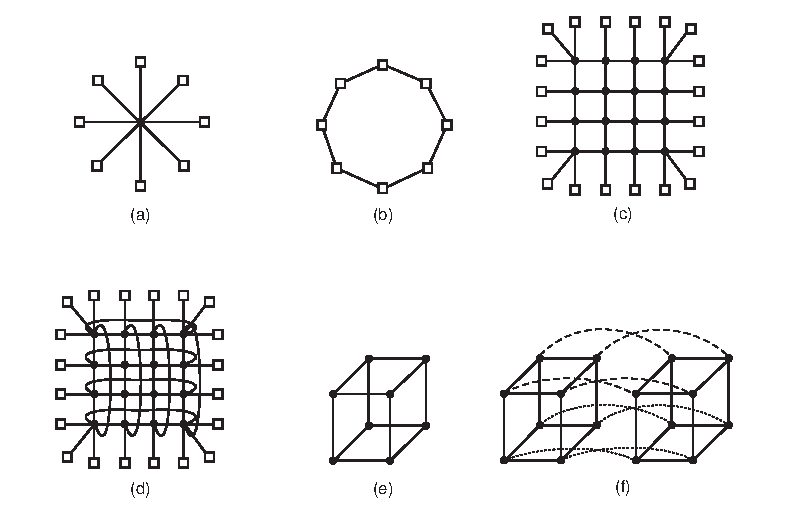
\includegraphics[width=.9\linewidth, keepaspectratio]{topologia.pdf}
  \fonte{\cite{TanenbaumMordenOS}.}
\end{figure}

Topologias mais complexas, como a malha (\textit{grid} ou \textit{mesh}), mostrada na Figura \ref{fig:topologiamulticomputadores}(c), ou a \textit{double torus}, mostrada na Figura \ref{fig:topologiamulticomputadores}(d), são mais escaláveis do que as apresentadas anteriormente. Nessas topologias, os nós são conectados em \textit{switches} e estes são conectados entre si, formando um \textit{layout} de malha no sistema. Dentre as duas citadas, a \textit{double torus} é mais escalável devido a conexão entre nós nas arestas da rede, trazendo assim conexões extras ao sistema, o que aumenta a tolerância a faltas e o desempenho, já que o caminho entre estes nós se torna menor. Este tipo de rede possui uma propriedade chamada de diâmetro, que é o caminho mais longo entre dois nós. Para topologias bidimensionais como a malha, o diâmetro aumenta proporcionalmente a raiz quadrada do número de nós. \textit{Layouts} \textit{n} dimensionais, como mostrado na Figura \ref{fig:topologiamulticomputadores}(e) (tridimensional) e na Figura \ref{fig:topologiamulticomputadores}(f) (quadrimensional), são ainda mais escaláveis, já que o diâmetro diminui à medida que se aumenta o número de dimensões da rede, tendo como única desvantagem o custo elevado, devido ao grande número de ligações presentes entre nós e \textit{switches}.

A comunicação entre processos rodando em diferentes \CPUs, num multicomputador, se dá através da troca de mensagens entre estes. Basicamente, o \SO presente no multicomputador é o responsável por realizar essa troca, através de funções acessíveis somente a ele. Porém, bibliotecas podem fornecer abstrações a essas funções, tornando a troca de mensagens também disponível para os processos usuário e as simplificando, visto que abstraem toda uma lista de invocações de funções em uma única função. Essa troca de mensagens pode ser reduzida a duas funções, chamadas de \textit{send} e \textit{receive}. A função \textit{send} é responsável por enviar uma mensagem de uma \CPU para outra, passando parâmetros como o destino da mensagem e o endereço onde aquela mensagem se encontra. Já a função \textit{receive} é responsável por receber a mensagem, tendo como parâmetros, por exemplo, o endereço de onde a mensagem será lida e o endereço onde será armazenada. Por fim, essas funções podem ser síncronas, bloqueando o processo que envia ou recebe a mensagem até que a operação seja concluída, ou assíncronas, não bloqueando o processo que realizou tal operação.

\section{\mppa}
\label{sec:mppa256}

\begin{figure}[tb]
  \centering
  \caption{Visão arquitetural simplificada do \mppa.}
  \label{fig:mppa256overview}
  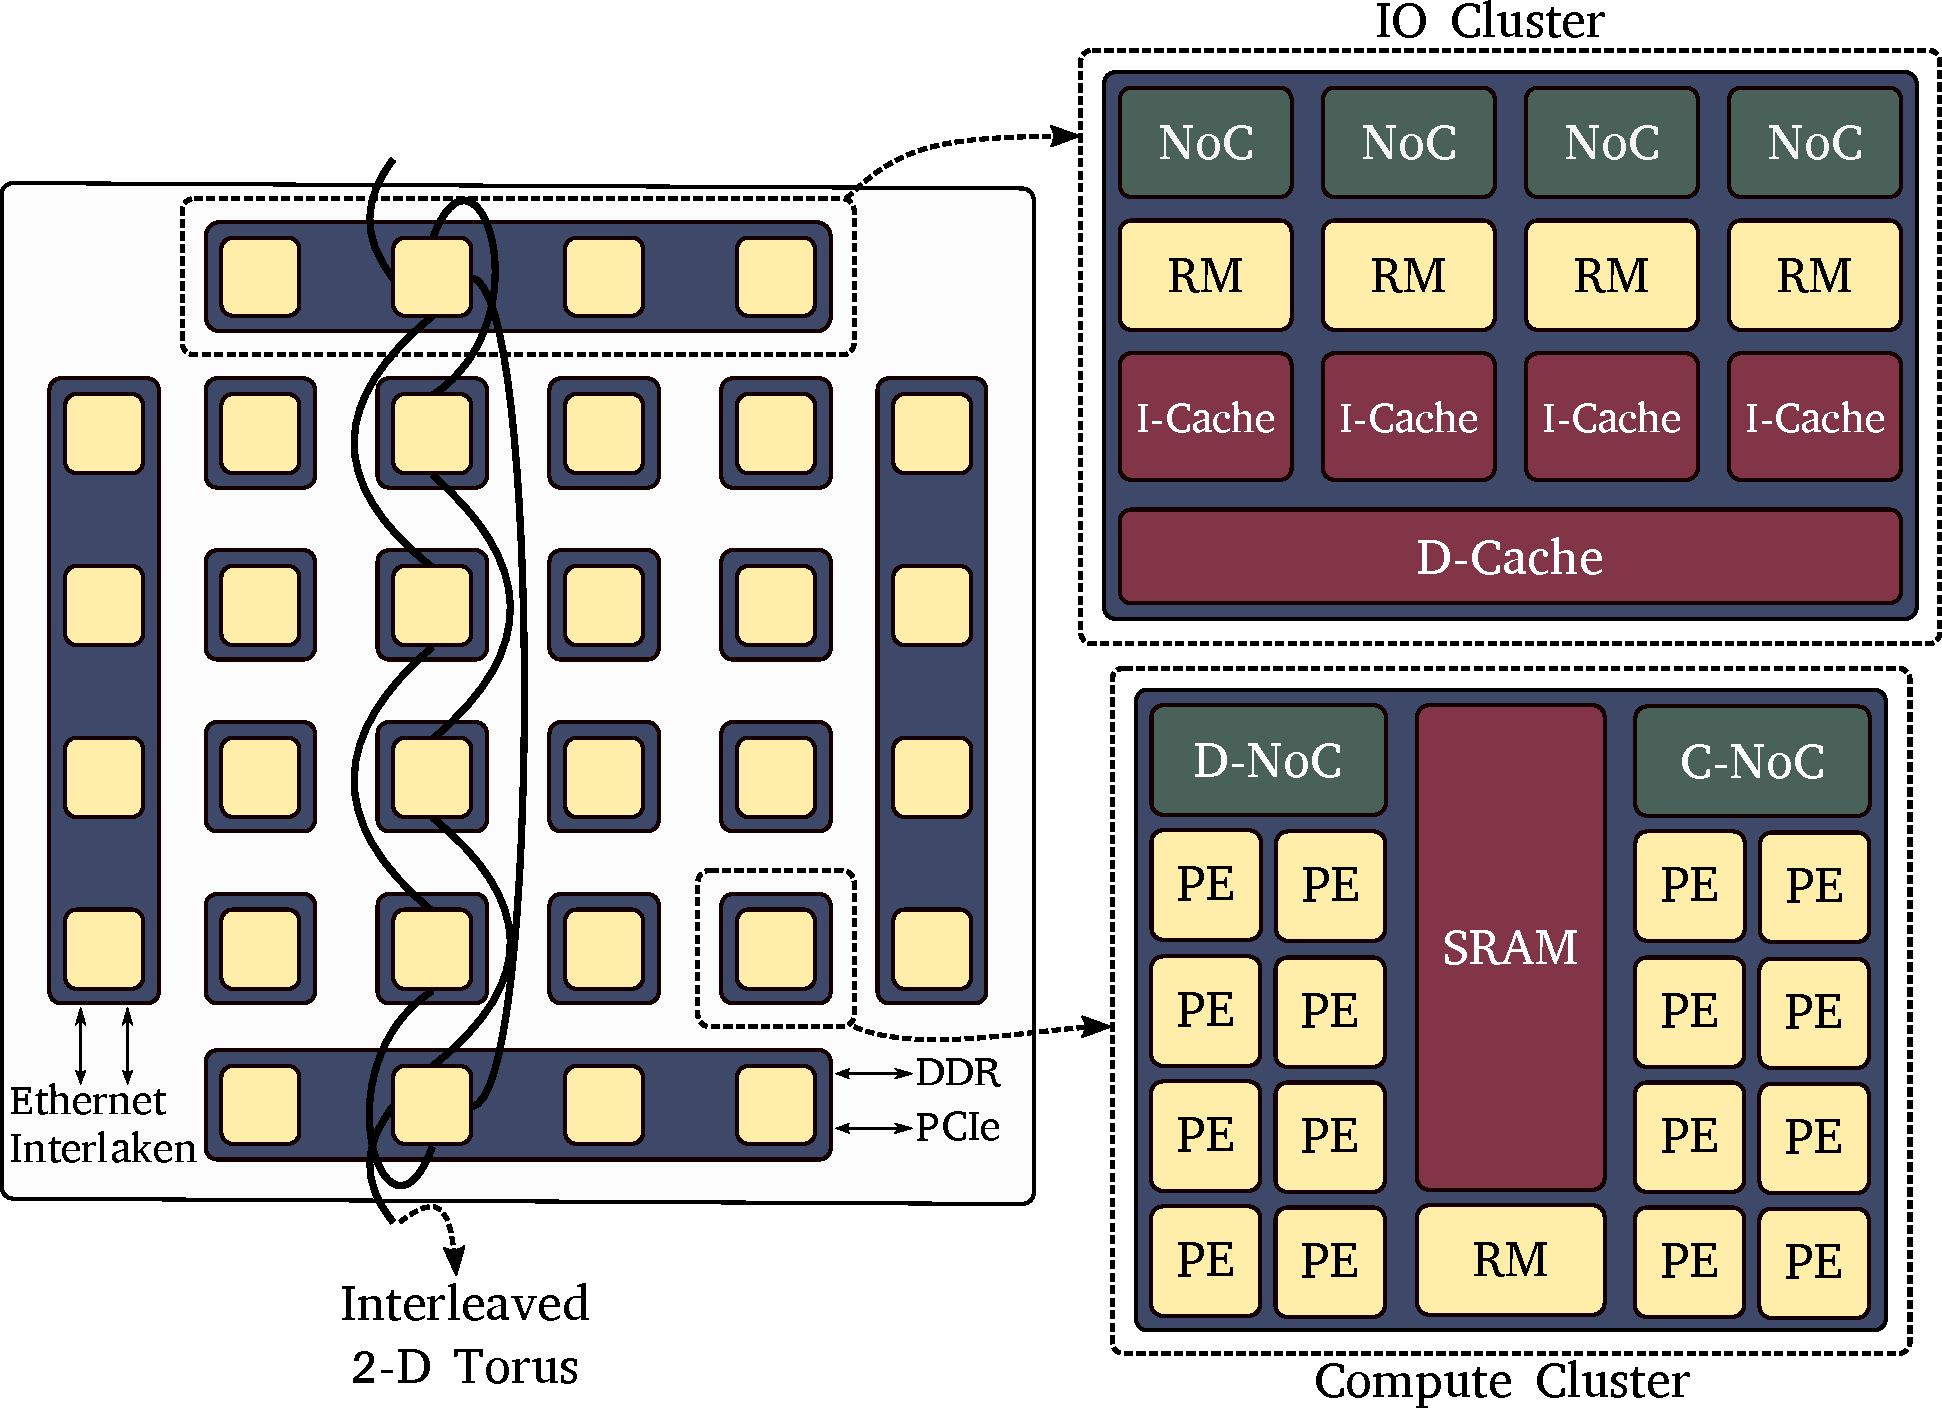
\includegraphics[width=.7\linewidth, keepaspectratio]{mppa-overview.pdf}
  \fonte{\cite{Penna2018OS}.}
\end{figure}

Desenvolvido pela empresa francesa Kalray, o \mppa é um processador de baixa potência que reflete o estado da arte dos \manycore. Uma visão geral do processador é mostrada na Figura \ref{fig:mppa256overview}. O \mppa possui 16 \CCs e 4 \clusters de \IO. Cada \CC possui: \textbf{(i)} 16 núcleos para executar \textit{threads} de usuário em modo ininterrupto e não preemptivo, os quais atuam com frequência de 400 MHz; \textbf{(ii)} um gerenciador de recursos responsável por executar
o sistema operacional e gerenciar comunicações; \textbf{(iii)} uma memória compartilhada de 2MB, possibilitando alta largura de banda e taxa de transferência entre núcleos de um mesmo \cluster; e \textbf{(iv)} dois controladores de Rede-em-Chip (\NoC), um para dados e outro para controle. Cada núcleo possui duas memórias \cache, uma para dados e outra para instruções. As \caches são associativas \textit{2-way} privadas e possuem 32kB \cite{Podesta2018Stencil}.

Por outro lado, \clusters de \IO realizam comunicações com dispositivos externos, onde dois destes apresentam acesso às memórias externas \textit{Low-Power Double Data Rate 3 (LPDDR3)} de 2GB. É importante salientar que um \CC não pode acessar diretamente os dados da memória de outros \clusters. Logo, o processador apresenta um modelo de memória distribuído \cite{Castro-Souza-CCPE:2016, Podesta2018Stencil}.

\section{Desenvolvimento de Aplicações Paralelas}
\label{sec:bibliotecasdevparalelo}

Durante o domínio de processadores \singlecore no mercado, para que uma aplicação ganhasse aumento em performance, bastava esta ser executada em um processador com maior frequência de \textit{clock}. Isso removia parte da responsabilidade do desenvolvedor em implementar melhorias na aplicação, já que bastava o \textit{upgrade} no hardware para obter essas melhorias. Nestes processadores, instruções são executadas de forma sequencial em um único núcleo. Já em processadores \multicore e \manycore, existem múltiplos núcleos executando diferentes instruções, possivelmente, de diferentes programas. Essa divisão de tarefas pode levar a diversos novos problemas, como \textit{deadlock} ou condições de corrida.

Diversas \APIs voltadas a programação paralela foram criadas para simplificar tanto a solução desses problemas como o desenvolvimento de aplicações que implementam paralelismo. Abaixo serão apresentadas duas das mais conhecidas \APIs para multiplataformas, a \OpenMP e o \MPI, assim como duas \APIs específicas para o \mppa, a \ASYNC e a \IPC.

\subsection{Bibliotecas multiplataforma}
\label{sec:bibliotecasmultiplataforma}

\subsubsection{Open Multi-Processing}
\label{sec:openmp}

A \OpenMP é uma das bibliotecas mais utilizadas para implementação de aplicações paralelas nas linguagens C, C++ e Fortran. Sua fama vem, principalmente, da abstração que a \API fornece, sendo possível ser utilizada em inúmeras plataformas. Por ser uma \API voltada ao \textit{multithreading}, utiliza-se do compartilhamento de memória entre as \threads de um mesmo programa para criar beneficios ao desenvolvedor, como variáveis de ambiente.

Esta biblioteca é centrada no modelo \textit{fork-join} (Figura \ref{fig:forkjoin}), onde, em determinados momentos do fluxo de execução de uma aplicação, temos a \thread principal instanciando outras \threads através de diretivas de compilação fornecidas pela própria \API, as quais serão executadas de forma independente, paralelamente ou concorrentemente entre si. A \thread principal também realiza uma sincronização com as \threads criadas através de uma barreira implícita, aguardando o término de todas as \threads para continuar com a execução. A criação de novas \threads se dá ao atingir uma região paralela, definida por algumas diretivas de compilação, como \texttt{\#pragma omp parallel for}, que paraleliza a execução de um \textit{loop} entre múltiplas threads. O código \ref{lst:parallelloop} produz, de forma paralela, um array com 10 posições, onde cada posição armazena um inteiro igual ao índice daquela posição.


\begin{figure}[tb]
  \centering
  \caption{Esquema do modelo \textit{fork-join}.}
  \label{fig:forkjoin}
  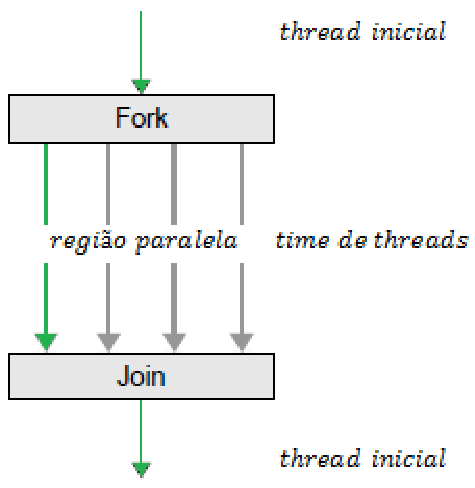
\includegraphics[width=.3\linewidth, keepaspectratio]{forkjoin.pdf}
  \fonte{\cite{forkjoinarticle}.}
\end{figure}

\begin{listing}[tb]
\caption{Execução de um \textit{loop} de forma paralela.}
\label{lst:parallelloop}
\begin{minted}[highlightlines={4}]{c}
static void createArray() {
  int array[max], index;
  int index_max = 10;
  #pragma omp parallel for
  for (index = 0; i < index_max; index++)
    array[index] = index;
}
\end{minted}
\fonte{o autor.}
\end{listing}

As diretivas \texttt{private, default e reduction} permitem, na sequência, definir quais variáveis terão escopo privado, qual será o escopo padrão das variáveis, e qual variável será feito uma redução sobre e qual será o tipo de redução (reduções são operações primitivas seguras sobre uma variável compartilhada entre múltiplas \threads). O código \ref{lst:reductionloop} é parte de uma das aplicações do \capb, a \textit{Friendly Numbers}, e utiliza essas três diretivas para realizar uma contagem paralela, a qual será armazenada na variável \texttt{partial\_friendly\_sum}. Ambas implementações mostram que, com a adição de uma única linha, muda-se completamente o fluxo de execução do programa, sendo esta a maior vantagem da \OpenMP.

\begin{listing}[tb]
\caption{Leitura e armazenamento seguro em variável compartilhada entre \threads.}
\label{lst:reductionloop}
\begin{minted}[highlightlines={6}]{c}
static int partial_friendly_sum = 0;
...
static void countFriends() {
  int i; /* Loop indexes. */

  #pragma omp parallel for private(i) default(shared) reduction(+: partial_friendly_sum)
  for (i = offset; i < offset + tasksize; i++) {
    for (int j = 0; j < i; j++) {
      if ((allTasks[i].num == allTasks[j].num) && (allTasks[i].den == allTasks[j].den))
        partial_friendly_sum++;
    }
  }
}
\end{minted}
\fonte{o autor.}
\end{listing}

Também pode-se definir qual será o nível de trabalho de cada \thread com a diretiva \texttt{schedule}. Através desta diretiva, definem-se três tipos de escalonamentos para as \threads: \texttt{static}, \texttt{dynamic} e \texttt{guided}. Com o \texttt{static}, todas as \threads irão receber a mesma quantidade de trabalho, sendo este o escalonamento padrão. Já a diretiva \texttt{dynamic} é utilizada quando as iterações podem ter uma grande diferença no seu tempo de execução, realizando uma atribuição dinâmica de tarefas, onde cada \thread recebe uma nova tarefa ao terminar a iteração atual. Por fim, \texttt{guided} é similar ao \texttt{dynamic}, porém, a \thread começa recebendo um grande número de iterações, e se adaptando conforme executa, recebendo mais ou menos iterações, dependendo do tempo que leva para executá-las.

\subsubsection{Message Passing Interface}
\label{sec:mpi}

\begin{listing}[tb]
\caption{Exemplo de uma aplicação usando a MPI.}
\label{lst:programmpi}
\begin{minted}[highlightlines={10,14,17}]{c}
int main(int argc, char **argv) {
  int rank, size;

  char mensagem_bcast[25] = "Transmitindo um broadcast";
  char mensagem_bcast_recebido[18];

  MPI_Init(argc, argv);
  MPI_Comm_rank(MPI_COMM_WORLD, &rank);
  MPI_Comm_size(MPI_COMM_WORLD, &size);
  MPI_Bcast(&mensagem_bcast, 25, MPI_CHAR, 0, MPI_COMM_WORLD);

  if (rank > 0) {
    mensagem_bcast_recebido[18] = "Broadcast recebido";
    MPI_Send (&mensagem_bcast_recebido, 18, MPI_CHAR, 0, 0, MPI_COMM_WORLD);
  } else if (rank == 0) {
    for (int i = 1; i < size; i++)
      MPI_Recv(&mensagem_bcast_recebido, 18, MPI_CHAR, i, 
        MPI_ANY_TAG, MPI_COMM_WORLD, MPI_STATUS_IGNORE);
  }

  MPI_Finalize();
  return 0;
}
\end{minted}
\fonte{o autor.}
\end{listing}

Diferentemente da \OpenMP, o \MPI é baseada no modelo \SPMD, onde um mesmo programa é executado por diferentes processos, cada qual tendo acesso a uma determinada região de memória. Assim, o \MPI é usada em supercomputadores para abstrair a difícil tarefa de implementar nestes o paralelismo através da troca de mensagens entre processos em baixo nível. Com esta \API de alto nível, implementar o envio e recebimento de mensagens torna-se algo tão simples como chamar uma função, já que o \MPI abstrai diversas etapas em uma única função. A \API também adiciona identificadores únicos e um grupo de comunicação para cada processo, os quais são usados como parâmetros em diversas de suas funções. Além disso, determinadas funções podem ser executadas de forma síncrona ou assíncrona, aumentando o desempenho da aplicação.

Um fluxo simples de implementação utilizando o \MPI começa com a função \texttt{MPI\_Init()}, que inicia o ambiente de execução \MPI. Na sequência, obtém-se o \textit{id} de um processo através da função \texttt{MPI\_Comm\_rank()}, a qual recebe um comunicador, geralmente o comunicador padrão \texttt{MPI\_COMM\_WORLD}, como primeiro parâmetro e o endereço da variável que será armazenado o \textit{id} do processo como segundo. Também é possível obter o número máximo de processos em um grupo de comunicação através da função \texttt{MPI\_Comm\_size()}, a qual recebe no primeiro parâmetro um comunicador e no segundo o endereço da variável em que será armazenado este número. Além disso, existem as funções de envio e recebimento de mensagens, \texttt{MPI\_Send()} e \texttt{MPI\_Recv()}, as quais ambas recebem parâmetros como o buffer de dados sobre o qual será realizado a leitura ou armazenamento da mensagem, a quantidade de dados, o tipo do dado e o \textit{id} do processo que realizará o envio ou recebimento da mensagem, além de alguns parâmetros adicionais. Por fim, a função \texttt{MPI\_Finalize()} termina a execução do ambiente \MPI.

Ao contrário das funções \texttt{MPI\_Recv()} e \texttt{MPI\_Send()}, que são voltadas para comunicação entre dois processos, funções como \texttt{MPI\_Bcast()} e \texttt{MPI\_Barrier()} são feitas para que haja comunicação entre um grupo de processos. Com a \texttt{MPI\_Bcast()} define-se o envio de uma mensagem de um processo para todos os outros processos associados a um grupo de comunicação. Já com a \texttt{MPI\_Barrier()} cria-se uma barreira, onde um certo processo, ao chegar nesta barreira, aguarda todos os outros processos de um grupo de comunicação chegarem nela antes de continuar sua execução.

O código \ref{lst:programmpi} mostra um exemplo de implementação simples usando o \MPI. Neste exemplo, na linha 11 o processo com \textit{id} igual a 0 envia um \textit{broadcast} para todos os outros processos, os quais respondem na linha 16 ao processo de \textit{id} 0, que recebe esta resposta na linha 19. Assim, as linhas 18-20 são executadas somente pelo processo com \textit{id} igual a 0, enquanto que as linhas 14-16 são executadas por processos com \textit{id} maior que 0. 

\subsection{Bibliotecas específicas para o \mppa}
\label{sec:bibliotecasespecificasmppa}

Na arquitetura do \mppa existem \clusters que gerenciam outros \clusters, chamados de mestres, e \clusters específicos para a realização de computações, chamados de escravos. Por isso, as bibliotecas do processador fornecem funções voltadas a implementação de aplicações do tipo \textit{mestre/escravo}, exemplificado na Figura \ref{fig:masterslave}, sendo uma das principais diferenças do processador para um x86 a divisão do programa em duas partes, cada uma compilada para um dos dois tipos de \clusters. Ao ativar um \cluster, associa-se um processo a ele, logo, a inicialização de \CCs acontece através de um processo mestre citando explicitamente em sua implementação o caminho do código binário que será executado no \CC. Cada processo escravo pode criar até 16 \threads do tipo POSIX, cada uma sendo executada em um núcleo diferente dentro daquele \cluster. Ambas \ASYNC e \IPC seguem esses conceitos na implementação de suas abstrações, porém, por ser mais nova, a \ASYNC permite uma abstração maior que a \IPC. 

\begin{figure}[tb]
  \centering
  \caption{Fluxo de uma aplicação seguindo o modelo \textit{mestre/escravo} no \mppa.}
  \label{fig:masterslave}
  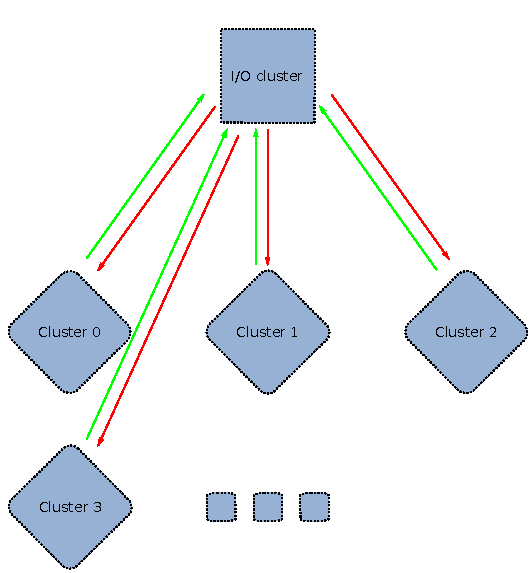
\includegraphics[width=.4\linewidth, keepaspectratio]{mppamasterslave.pdf}
  \fonte{Documentação do MPPA sobre IPC.}
\end{figure}

Com a \IPC, processos mestres localizados em um dos quatro \clusters de \IO conseguem \textit{spawnar} outros processos nos \CCs passando argumentos tradicionais, como \texttt{argc} e \texttt{argv}. Porém, toda a lógica de comunicação e sincronização sobre a rede \NoC é abstraída através da realização de operações sobre descritores de arquivos e através do uso das diretivas do padrão POSIX IPC. O \textit{design} da API é baseado no modelo \textit{pipe-and-filters} \cite{softwarecomponentmodels}, onde os processos POSIX são os componentes atômicos e os objetos de comunicação são as conexões. Além disso, os objetos de comunicação possuem portas de transmissão e recepção de dados, chamadas de portais, as quais são abertas em dois possíveis modos, \texttt{O\_WRONLY} (somente escrita) ou \texttt{O\_RDONLY} (somente leitura), através da função \texttt{mppa\_open()}, que recebe no primeiro parâmetro o \textit{path} para o descritor de arquivo de um determinado portal e no segundo o modo no qual será aberto.

Abrindo portais de comunicação específicos para cada \cluster, um para leitura e outro para escrita, e definindo quais \clusters ficarão em cada ponta desses portais, pode-se implementar uma aplicação que segue um fluxo semelhante a Figura \ref{fig:mppaipcflow}. Nela, o processo mestre \textit{spawna} dois processos escravos, os quais abrem portais que definem um caminho para o \cluster que os \textit{spawnou}. Um destes processos não faz uso da função \texttt{mppa\_read()} pois recebeu todos os dados necessários através dos parâmetros passados pelo processo de \IO na chamada a função \texttt{mppa\_spawn()}. Assim, este processo só precisa realizar a computação sobre aqueles dados e devolver o resultado para o \cluster de \IO através do portal que os liga, usando a função \texttt{mppa\_write()}. Já o outro \cluster faz uso da função \texttt{mppa\_read()} para ler dados enviados pelo processo mestre, mas não envia de volta nenhuma informação. Após realizar suas tarefas, os \CCs precisam fechar os descritores de arquivo dos portais que foram abertos e usados, o que é feito através da função \texttt{mppa\_close()}. Por fim, o processo mestre precisa esperar o término da execução dos processos escravos antes de continuar a sua execução, o que é feito com a função \texttt{mppa\_waitpid()}.

\begin{figure}[tb]
  \centering
  \caption{Fluxo de uma aplicação usando funções do tipo POSIX da IPC no \mppa.}
  \label{fig:mppaipcflow}
  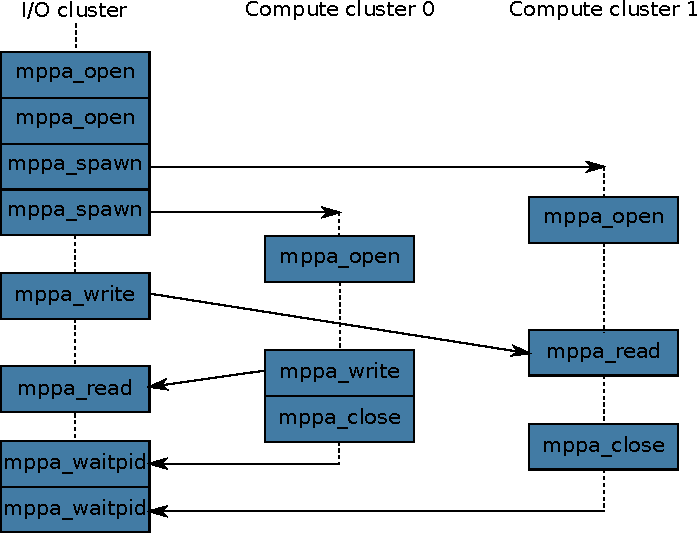
\includegraphics[width=.6\linewidth, keepaspectratio]{mppaipcflow.pdf}
  \fonte{Documentação do MPPA sobre IPC.}
\end{figure}

Baseada em princípios de comunicação unilateral, os quais são aplicados em diversas \APIs usadas em supercomputadores, como a \API PNNL ARMCI \cite{armciapproach}, a \ASYNC é organizada em diversos conceitos que permitem abstrair ainda mais a implementação de paralelismo no \mppa. Dentre esses conceitos, pode-se citar três mais importantes: \textbf{(i)} segmentos de memória, ou seja, memória que não é diretamente acessível através de um dos núcleos de um \cluster; \textbf{(ii)} operações \texttt{PUT/GET}, as quais possuem diversos modos de realização, como linear, espaçada, por etapas e em blocos 2D ou 3D; e \textbf{(iii)} o modo assíncrono como as operações \texttt{PUT/GET} são realizadas, significando que essas funções retornam assim que completam a escrita ou leitura sobre uma porção de memória, não realizando qualquer tipo de sincronização com algum possível \textit{cluster} que irá receber aquela informação.
 
\begin{figure}[tb]
  \centering
  \caption{Fluxo de uma aplicação usando a API ASYNC no \mppa.}
  \label{fig:mppaasyncflow}
  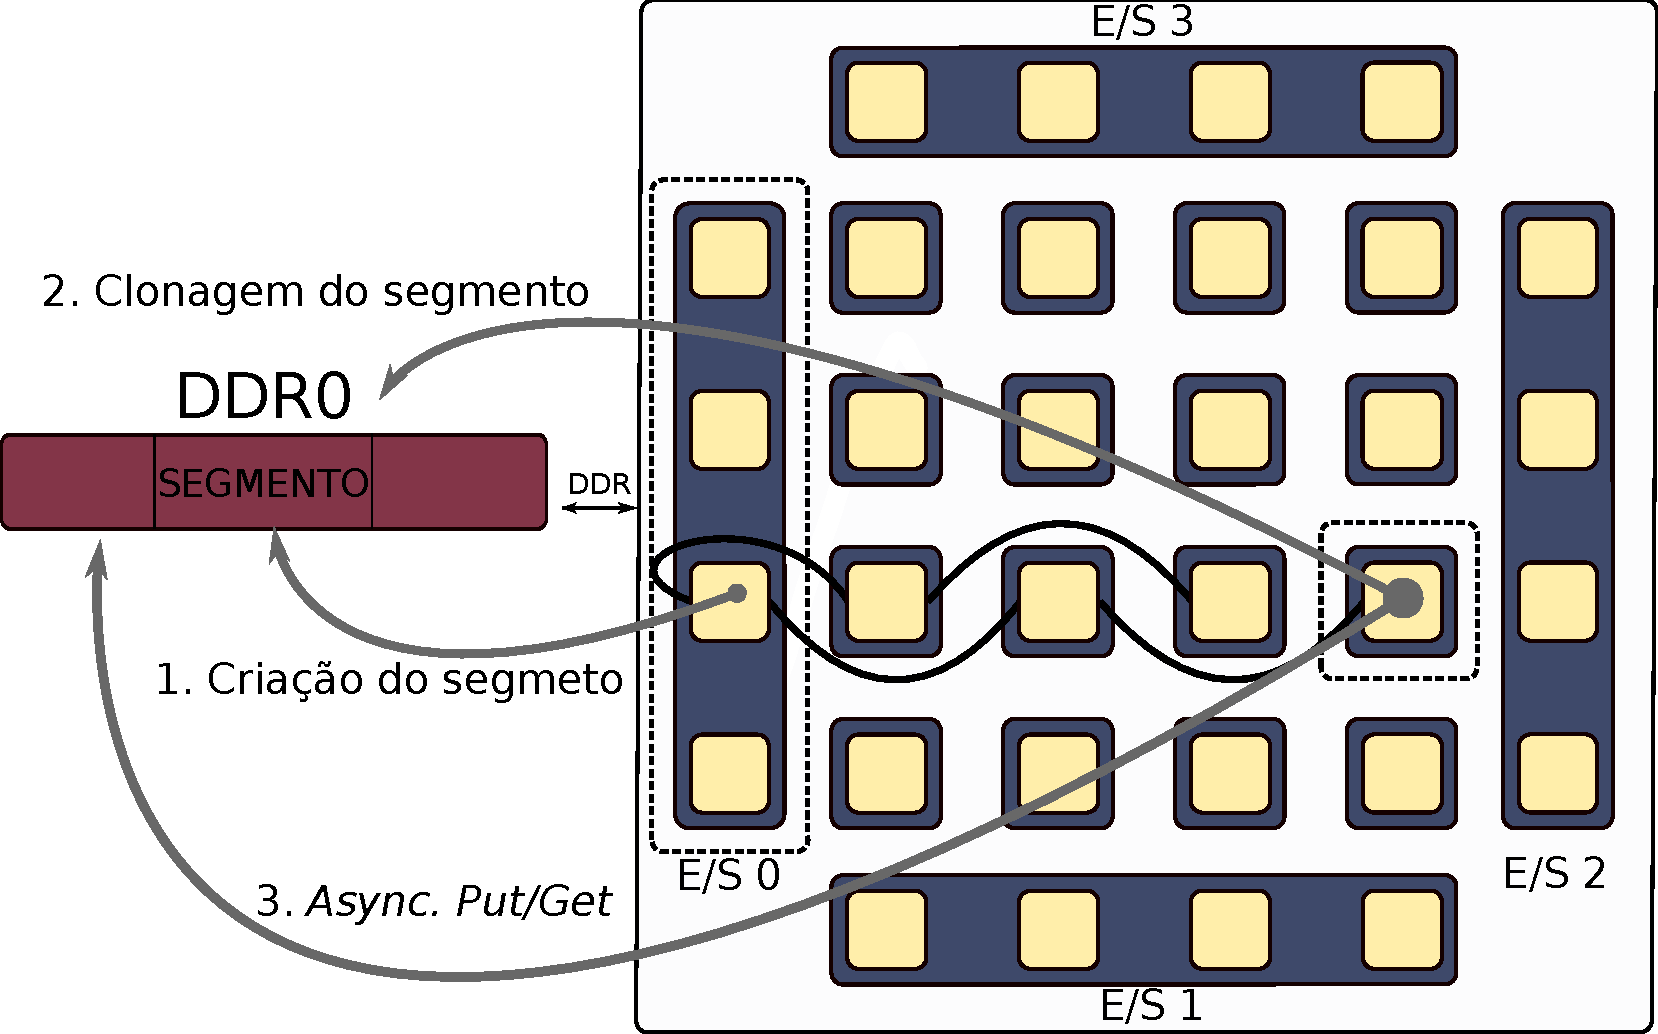
\includegraphics[width=.6\linewidth, keepaspectratio]{mppaasyncflow.pdf}
  \fonte{o autor.}
\end{figure}

Na figura \ref{fig:mppaasyncflow}, onde os \clusters são representados por quadrados amarelos, é demonstrado o fluxo de implementação do paralelismo entre um processo mestre e um \CC ao usar a \ASYNC. Primeiramente um \cluster de \IO cria um segmento sobre uma porção de dados localizados na sua memória local através da função \texttt{mppa\_async\_segment\_create()}, associando a ele um identificador único do tipo \texttt{unsigned long long}. Após a criação do segmento, um \cluster de computação deve clonar esse segmento através da função \texttt{mppa\_async\_segment\_clone()}, usando, entre outros parâmetros, o identificador do segmento desejado. Chamadas essas duas funções, operações do tipo \texttt{PUT/GET} podem ser realizadas sobre o segmento através das funções \texttt{mppa\_async\_put()} e \texttt{mppa\_async\_get()}. Além disso, é preciso inicializar o contexto antes de realizar qualquer uma dessas operações, o que é feito com a função \texttt{mppa\_async\_init()}, e finalizar este contexto após realizar todas as operações necessárias, o que é feito com a função \texttt{mppa\_async\_final()}.

Operações \texttt{PUT} devem ser feitas com cuidado, caso contrário podem sobrescrever operações anteriores que ainda não foram lidas por algum \cluster. Na versão \ASYNC do \capb, sincronizações são feitas através de operações \texttt{poke} sobre um segmento padrão construído na inicialização do contexto da \API. Essas sincronizações são definidas através de macros, que são expandidas para chamadas as funções \texttt{mppa\_async\_poke()} e \texttt{mppa\_async\_evalcond()}, as quais, respectivamente, alteram um valor remoto do tipo \texttt{long long} e aguardam uma expressão booleana se tornar verdadeira antes de continuar a execução. Os códigos \ref{lst:macrossyncio} e \ref{lst:macrossynccc} mostram como são definidas essas macros em um \cluster de \IO e em um \CC, respectivamente.

\begin{listing}[tb]
\caption{Definição das macros de sincronização em um \cluster de E/S.}
\label{lst:macrossyncio}
\begin{minted}{c}
/* Synchronization between slaves and IO. */
#define send_signal(i)                                     \
poke(mppa_async_default_segment((i)), sig_offsets[(i)], 1) \

/* Synchronization between slaves and IO. */
#define wait_signal(i) {                                           \
waitCondition(&cluster_signals[(i)], 1, MPPA_ASYNC_COND_EQ, NULL); \
cluster_signals[(i)] = 0;                                          \
}   
\end{minted}
\fonte{o autor.}
\end{listing}

\begin{listing}[tb]
\caption{Definição das macros de sincronização em um \cluster de computação.}
\label{lst:macrossynccc}
\begin{minted}{c}
/* Synchronization between slaves and IO. */
#define send_signal()                        \
poke(MPPA_ASYNC_DDR_0, sigback_offset, 1) \

/* Synchronization between slaves and IO. */
#define wait_signal() {                                 \
waitCondition(&io_signal, 1, MPPA_ASYNC_COND_EQ, NULL); \
io_signal = 0;                                          \
}     
\end{minted}
\fonte{o autor.}
\end{listing}

\chapter{Trabalhos Correlatos}
\label{ch:trabcorrelatos}

O tema central deste trabalho é de grande interesse por parte da comunidade científica de \HPC, existindo inúmeras pesquisas voltadas a medir o desempenho de processadores \multicore, \manycore e \chips \FPGA, as quais são diretamente relacionadas a esta. Neste capítulo serão apresentados algumas pesquisas científicas voltadas a medição de parâmetros de desempenho de processadores que utilizam uma dessas duas arquiteturas.

\textit{Nabi} \etal \cite{nabifpgabenchmark} implementaram uma versão do \bench STREAM para arquiteturas \FPGA, \GPUs e \CPUs, chamando-o de STREAM-Multiplataforma, para dar foco a portabilidade de sua versão. O \bench STREAM original foi desenvolvido em 1995 por \textit{McCalpin} \etal \cite{mccalpinstreambench} e é um dos \benchs mais utilizados para medir a largura de banda da memória em computadores. A principal contribuição deste trabalho é a introdução de um \bench que faça esse tipo de medição em dispositivos \FPGA, já que faltam \benchs desse tipo para estes dispositivos. Além disso, parâmetros genéricos e específicos para certas arquiteturas foram introduzidos na nova versão, os quais afetam diretamente a largura de banda da memória. Os autores afirmam que, sendo esta largura de banda um dos principais gargalos das aplicações \HPC \cite{asanoviclandscapeparallel}, este \bench possibilita mais um passo na direção de tornar convencional o uso de placas \FPGA.

Já \textit{Bennett} \etal \cite{bennettqcdbench} desenvolveram um \bench para avaliar a aptidão de um supercomputador ao executar simulações de modelos da física quântica que vão além do modelo padrão. Grande parte dos \benchs dessa área são derivados do modelo Quantum ChromoDynamics (QCD), que descreve a forte interação entre \textit{quarks} e \textit{gluons}. Porém, este modelo não tem a flexibilidade necessária para examinar outros que o estendem, como é o caso dos modelos da Teoria de Gauge, que inclui o QCD. Assim, a inovação deste \bench é ser derivado de implementações que simulam modelos da Teoria de Gauge, que é mais extensa. 

Dentre os \benchs clássicos da comunidade de \HPC, o NAS Parallel Benchmark \cite{baileynasbench} se destaca por ter sido concebido puramente através de algoritmos, descrito por seus autores como um \bench com especificação de papel e caneta. Segundos os autores, optar por este caminho é uma maneira de evitar grande parte das dificuldades que uma implementação convencional de um \bench para sistemas \HPC enfrenta. Originalmente 7 \kernels foram descritos para o NAS, os quais simulam diferentes cargas de trabalho encontradas em aplicações \HPC. Todos estes \kernels usam ou uma \API de comunicação entre processos, como a \MPI, ou uma \API para sistemas com memória compartilhada, como a \OpenMP.

Outro \bench clássico para aplicações CUDA + \MPI é o OMB-GPU \cite{bureddyomb}, que estende o OSU Micro-Benchmarks (OMB) adicionando \kernels que avaliam a performance de comunicações \MPI em sistemas de \clusters de \GPUs. O OMB-GPU surgiu durante o crescimento no uso de \GPUs em supercomputadores, devido a necessidade de um \bench padronizado para avaliar as novas bibliotecas \MPI que foram desenvolvidas para suportar comunicações \MPI nesses novos sistemas. Com o desenvolvimento da \UM para aplicações CUDA (tecnologia que mescla \textit{software} e \textit{hardware} para criar um espaço de endereço único e acessível por qualquer \GPU ou \CPU de um sistema), houve a necessidade de um novo \bench específico para os sistemas que passaram a utilizar essa tecnologia, já que os \benchs clássicos da época, como o OMB ou o OMB-GPU, não eram aptos para isso, pois não capturavam corretamente o comportamento do driver CUDA neste novo contexto. Assim, \textit{Manian} \etal desenvolveram o OMB-UM \cite{maniancudaum}, uma extensão do OMB para suportar aplicações CUDA + \MPI + \UM.

Diferentemente dos \benchs anteriores, \textit{Kelly} \etal \cite{kellynwsc} desenvolveram o \bench NWSC para testar um supercomputador especifico, o NCAR-Wyoming Supercomputing Center (NWSC), que estava sendo construído para suprir as necessidades computacionais de aplicações \HPC de 5 domínios científicos: \textbf{(i)} Física Atmosférica; \textbf{(ii)} Clima Espacial; \textbf{(iii)} Oceanografia; \textbf{(iv)} Modelagem de Subsuperfícies; e \textbf{(v)} Ciência Computacional, Estatística e Matemática. Este supercomputador seria o próximo sistema \HPC do Centro Nacional de Pesquisas Atmosféricas dos Estados Unidos, suportando grande parte da necessidade de poder computacional da comunidade científica de \HPC, logo, viu-se a necessidade de construção de um \bench específico para avaliá-lo.

Dentre as mais recentes pesquisas voltadas ao desenvolvimento de \benchs para a área de \HPC temos o Mirovia, um \bench desenvolvido por \textit{Hu} \etal \cite{miroviabenchmark} para tirar proveito de arquiteturas de \GPUs modernas, medindo de forma precisa os atuais sistemas heterogêneos, com processadores \multicore, \manycore e \GPUs. O Mirovia foi desenvolvido na necessidade de um \bench que levasse em conta as novas tecnologias que esses sistemas possuem, como a memória unificada, já que os \benchs clássicos, como o Rodinia \cite{rodiniabench} ou o SHOC \cite{shocbench}, foram desenvolvidos antes do surgimento destas. Além disso, devido ao crescente interesse em redes neurais e aprendizagem profunda, alguns \kernels com foco nesta área foram adicionados. Assim, o Mirovia tem como base \kernels de \benchs clássicos e adiciona \kernels de aplicações de maior interesse atual para melhor caracterizar os sistemas heterogêneos modernos.

Por fim, \textit{Tian} \etal \cite{tianbench} desenvolveram o BigDataBench-S, um \bench que avalia a performance de sistemas de gerenciamento de \textit{bBig Data}. Os autores ressaltam que o número de dados gerados por aplicações científicas é cada vez maior e que os atuais \benchs desse contexto foram feitos para sistemas que focam ou na Internet ou em alguma área científica específica. Assim, o BigDataBench-S surge como um \bench representativo para avaliar os sistemas de gerenciamento e análise de dados gerados por aplicações, equipamentos e dispositivos de propósito científico.

\chapter{Desenvolvimento}
\label{ch:desenvolvimento}

Para a realização deste trabalho, foram feitas dois tipos de alterações em todas as aplicações do \capb. Primeiro, criou-se uma nova versão de cada aplicação, a qual teve parte de ou toda sua lógica de processamento alterada para que pudesse utilizar a \API \ASYNC. Após isso, alterou-se as versões antigas, que usam a \API \IPC, para que ficassem equivalente as novas aplicações em relação ao seu fluxo de processamento. Nesta seção serão mostradas todas as alterações feitas em cada aplicação e em cada etapa. Uma descrição mais detalhada de cada um dos \kernels pode ser encontrada no trabalho de \textit{Souza} \etal \cite{Castro-Souza-CCPE:2016}.

\section{Alterações na Friendly Numbers}
\label{sec:alteracoesfn}

A primeira aplicação portada com a \ASYNC foi a \FN, tendo pequenas alterações devido a sua baixa complexidade. Em ambas as versões, existe um array de tamanho fixo que define as tarefas de cada \cluster segundo intervalos de \offsets, onde em cada posição existem três variáveis do tipo \texttt{int} agrupadas em uma \texttt{struct}. Resumindo, o \cluster de \IO define um intervalo de números e seta cada número na variável \texttt{number} de cada \texttt{struct}, enquanto que os \CCs devem calcular as variáveis \texttt{num} e \texttt{den}. O código \ref{lst:structitemtask} detalha como é feita a implementação de ambos array e \texttt{struct}.

\begin{listing}[h]
\caption{Definição das taréfas por  parte do \cluster de IO.}
\label{lst:structitemtask}
\begin{minted}{c}
/* Items to be sent to slaves */
typedef struct {
    int number; /* Number    */
    int num;  /* Numerator   */
    int den;  /* Denominator */
} Item;    

#define MAX_TASK_SIZE 65536

static Item tasks[MAX_TASK_SIZE];
\end{minted}
\fonte{o autor.}
\end{listing}

A versão \ASYNC possibilitou a redução de grande parte do fluxo de operações desta aplicação. Anteriormente, era necessário explicitamente realizar operações de envio e recebimento de mensagens no \cluster de \IO, através das macros \texttt{data\_send()} e \texttt{data\_receive()}, sendo essas operações totalmente bloqueantes. Com a introdução dos segmentos pela \API \ASYNC, duas linhas de código substituem ambas operações, ou seja, basta declarar um segmento e criá-lo, através da função \texttt{mppa\_async\_segment\_create()}, sobre o \textit{array} de tarefas. Assim, qualquer \CC que clona-lo poderá acessar seu conteúdo e modificá-lo, sendo essas modificações totalmente acessíveis ao cluster de \IO através do mesmo \textit{array} de tarefas.

Dessa maneira, os \CCs só são \textit{spawnados} depois que todas as tarefas estão definidas no \textit{array} e o segmento foi criado. Após \textit{spawnado}, um \cluster de computação só precisa fazer uma operação \texttt{GET} em um certo intervalo no segmento, processar os dados, e enviá-los de volta através de uma operação \texttt{PUT} no mesmo intervalo no segmento. Como cada \CC possui um intervalo de \offsets diferente, não há sobreposição de tarefas e não existe nenhuma condição de corrida sobre uma certa posição no segmento. Por fim, como as operações \texttt{PUT} dos \CCs alteram o array no qual o segmento foi definido no \cluster de \IO, não há necessidade do processo \master realizar um \texttt{GET} sobre aquele segmento, bastando acessar o \textit{array} de tarefas diretamente. Logicamente, se o processo \master ler o \textit{array} antes da hora, irá obter valores \texttt{null} para as variáveis \texttt{num} e \texttt{den}, logo, é feita uma única sincronização, onde os \clusters de \IO aguardam a sinalização dos \CCs de que determinada tarefa já foi computada e colocada em um certo intervalo do segmento, antes de ler aquele intervalo.

Mudanças sem relação com as \APIs também foram implementadas em ambas as versões. No código dos \slaves, existe uma função que computa a soma dos divisores de um número. Nesta função, era feito um \textit{loop} iniciando em 2 e terminando no número, onde em cada iteração verifica-se se o número daquela iteração era divisor do número passado como argumento para a função. Com a otimização, alterou-se o \textit{loop} para iterar até metade do número passado como argumento, já que, acima da metade, o único divisor de um número é ele mesmo. Outra otimização feita foi em relação ao paralelismo para verificar quais números tinham as variáveis \texttt{num} e \texttt{den} iguais. Na versão antiga utilizou-se \textit{POSIX Threads} para fazer uma soma parcial e depois uma redução na \textit{thread} principal, gastando mais de 50 linhas nessa lógica. Na nova versão, com a utilização de diretivas do \OpenMP, reduziu-se essas 50 linhas em 5, com um fluxo de execução muito mais fácil de ser entendido.

\section{Alterações na Features from Accelerated Segment Test}
\label{sec:alteracoesfast}

A versão antiga da \FAST sofreu otimizações em partes que ocupavam a maior porcentagem do seu tempo de execução. Nesta versão, o \cluster de \IO realizava o envio de tarefas aos \CCs através de iterações em um \texttt{for}, enquanto que os \CCs aguardavam as tarefas em um \texttt{while(true)}, recebendo, primeiramente, uma mensagem sinalizando se naquela iteração era necessário computar algo ou se poderia encerrar sua execução. Porém, como todas as variáveis utilizadas no \texttt{for} do processo \master poderiam ser passadas como argumento no momento de \textit{spawnar} um \CC, foi implementado isso em ambas as novas versões, o que resultou na eliminação de toda a lógica de enviar uma mensagem ao \slave para sinalizar se este deve ou não continuar sua execução. Assim, implementou-se um \texttt{for} com início e fim bem definidos no código do \slave, eliminando o \texttt{while(true)} deste e reduzindo de quatro para uma o número de mensagens que os \slaves recebem por iteração. Além disso, em ambas versões, reduziu-se de duas para uma o número de mensagens enviadas dos \slaves para o \master por iteração, pois na nova versão, em vez de retornar a cada iteração ambos o número de cantos detectados e parte da nova imagem, só é retornado o segundo, somando o primeiro em cada iteração e o retornando ao fim de todas elas.

Na versão \ASYNC foram criados 3 segmentos sobre os dados necessários para os \slaves. Primeiro, um segmento sobre a máscara a ser aplicada na imagem que se quer detectar os cantos, o qual todos os \CCs tem acesso completo. Em seguida, um sobre a imagem original e um sobre o \textit{array} que irá conter o resultado do filtro aplicado a esta imagem, os quais os \CCs só tem acesso a uma lista de intervalos de \offsets. Assim, nesta versão a otimização é ainda melhor, pois com toda a abstração que os segmentos trazem, a troca de mensagens cai pela metade, já que somente os \slaves precisam realizar operações \texttt{PUT} e \texttt{GET}, bastando ao \master criar os segmentos sobre os dados. Além disso, com as otimizações do parágrafo anterior, os \slaves agora sabem exatamente o número de operações que devem executar e, como conhecem os intervalos de \offsets que podem acessar dentro dos segmentos da imagem original e imagem filtrada, são totalmente autônomos para pegar e responder as tarefas nestes segmentos de forma totalmente assíncrona e paralela. Essa autonomia também se dá pois estes intervalos são diferentes para todos os \slaves, não havendo a repetição de nenhum intervalo em dois \CCs distintos, o que elimina a possibilidade de condições de corrida e permite um paralelismo com eficiência máxima.

\section{Alterações na Gausian Filter}
\label{sec:alteracoesgf}

Poucas foram as alterações da \GF, sendo esta a aplicação com menos modificações, dentre todas as outras. Quanto a versão \IPC, nada foi modificado. Já a versão \ASYNC seguiu a mesma lógica da versão \IPC, substituindo as chamadas das funções síncronas de envio e recebimento de mensagens para chamadas as funções assíncronas de \texttt{PUT} e \texttt{GET}. Para realizar esta substituição, foram criados dois segmentos de dados, sendo um sobre o \textit{array} que guarda a máscara a ser aplicada na imagem e outro sobre o \textit{array} que guarda o pedaço da imagem a ser trabalhado em determinada iteração, chamado de \textit{chunk}. Ambos podem ser completamente acessados pelos \slaves, porém, no segundo só é feito um acesso por vez. Assim, o método de comunicação de dados sobre este segmento é separado em duas etapas, as quais, dependendo do tamanho da imagem a ser aplicada o filtro, podem ou não acontecer diversas vezes durante a execução da aplicação. 

Na primeira etapa, o \cluster de \IO realiza somente escritas sobre o segmento, onde cada escrita é seguida de uma leitura por algum \CC, o qual armazena o que foi lido em sua memória local e sinaliza ao processo \master para prosseguir com a inserção da próxima tarefa para o próximo \CC. Já na segunda etapa, após terem feito toda computação sobre o \textit{chunk} que receberam, os \CCs aguardam o processo \master sinalizar que está na hora de escrever o dado calculado sobre o mesmo segmento em que foi recebido o \textit{chunk}, e, quando sinalizados, escrevem-no. Enquanto isso, o \cluster de \IO aguarda cada \CC sinalizar que tal dado já foi escrito no segmento. Apesar de complexo, este método é ligeiramente melhor que o da versão \IPC, visto que as operações \texttt{PUT} e \texttt{GET} de envio e recebimento de mensagens só são realizadas no lado dos \clusters de computação, já que no processo \master só é necessário copiar o dado do segmento para algum lugar dentro do \textit{array} que irá conter a nova imagem. Assim, similar às demais aplicações, a troca de mensagens é reduzida pela metade.

\section{Alterações na LU Factorization}
\label{sec:alteracoeslu}

A aplicação com maior número de modificações em sua lógica foi a \LU, principalmente por causa da implementação errônea do algoritmo na primeira versão. Basicamente, o algoritmo de decomposição LU transforma uma matriz \mathnormal{A} em duas matrizes, uma triangular inferior (\mathnormal{L}) e uma triangular superior (\mathnormal{U}), de modo que \mathnormal{A = L * U}. Porém, o erro da primeira versão foi implementar permutações de trocas de linha e coluna, as quais caracterizam outra decomposição, chamada de PLU e definida pela equação \mathnormal{P * A = L * U}, onde \mathnormal{P} é o agregado final de todas as matrizes de permutação aplicadas sobre A. Assim, funções de percorriam extensivamente a matriz em busca de um novo pivô e funções que trocavam linhas e colunas foram removidas. Além disso, blocos dentro da matriz eram enviados de forma errada aos \slaves, gerando um resultado final totalmente errado. A figura \ref{fig:rightandwrongblocks} mostra como um bloco de 9 elementos (3x3) deveria ser passado, segundo a matriz \mathnormal{B}, e como era passado primeira versão, segundo a matriz {A} (os blocos estão pintados em vermelho). Vale salientar que esse erro só foi possível pois a variável que guarda a matriz na verdade é um array unidimensional.

\begin{figure}[h]
  \centering
  \caption{Exemplo de um bloco passado a um \slave em cada versão da LU.}
  \label{fig:rightandwrongblocks}
  \[
    A=
    \begin{bmatrix}
      1  & 5  & 3  & 8  \\
      12 & \color{red} 7  & \color{red} 15 & \color{red} 12 \\
      \color{red}  3  & \color{red}  12 & \color{red}  92 & \color{red} 8 \\
      \color{red}  6  & \color{red}  9  & 3  & 1 
    \end{bmatrix}\quad
    B=
    \begin{bmatrix}
      1  & 5  & 3  & 8  \\
      12 & \color{red} 7  & \color{red} 15 & \color{red} 12 \\
      3  & \color{red} 12 & \color{red} 92 & \color{red} 8 \\
      6  & \color{red} 9  & \color{red} 3  & \color{red} 1 
    \end{bmatrix}
  \]
\end{figure}

Todos os erros citados no parágrafo anterior foram solucionados em ambas as versões. Quanto a versão \ASYNC, para tirar proveito desta \API foi criado um segmento sobre a matriz original e um segmento sobre um \textit{array} de tarefas. Deste modo, em uma certa iteração, um processo \slave consulta o segmento de tarefas usando seu próprio \textit{id} como \offset, recuperando um tarefa que contém, entre outras variáveis, os \offsets que serão aplicados para pegar um bloco no segmento da matriz. Quando um \CC não possui mais tarefas, o \cluster de \IO coloca uma mensagem de finalização no \offset deste \slave dentro do segmento de tarefas, o qual a recebe e finaliza sua execução. Devido aos dois segmentos citados acima, as operações \texttt{PUT} e \texttt{GET} são feitas somente pelos \CCs, enquanto que o processo \master só realiza sinalizações, quando coloca uma tarefa no segmento, e sincronizações, quando todos os \slaves finalizam uma iteração de computação.

\section{Alterações na K-Means}
\label{sec:alteracoeskm}

Diversas simplificações na lógica do \kernel \KM foram feitas. Primeiramente, devido a grande quantidade de dados enviados aos \CCs e a diferença nos tipos destes dados, resolveu-se adotar uma nova estratégia, desta vez utilizando o segmento padrão \texttt{MPPA\_ASYNC\_DDR\_0}, que é sempre criado na inicialização da \ASYNC, para o envio destes. Desta forma, através da função \texttt{mppa\_async\_malloc()}, cada \slave aloca uma porção de memória neste segmento para cada uma das variáveis que vão utilizar em suas iterações e comunicações. Esta função então retorna um \offset apontando para onde aquele espaço foi alocado dentro do segmento, e todos os \offsets são enviados para o processo \master, através de outro segmento especialmente criado para isso. Ao término desta primeira etapa, o processo \master saberá onde ler e escrever todos os dados no segmento padrão e, em etapas subsequentes, todas as comunicações dos dados computados serão feitas neste segmento, utilizando estes \offsets.

Pensando na otimização do envio e recebimento dos dados em cada iteração, o modelo de dados da aplicação também foi simplificado. Na versão original, os pontos eram definidos como \texttt{structs}, chamadas de vetores, contendo o tamanho (dimensão do vetor) e um ponteiro para os elementos (coordenadas do vetor). Porém, como todos os vetores possuem o mesmo tamanho, já que a dimensão é tratada globalmente, foi possível otimizar este modelo, inicializando todos os pontos em unico \textit{array} unidimensional. Desse modo, em um cenário com P pontos, todos com dimensão \mathnormal{X}, cada ponto ocupa \mathnormal{X} posições do \textit{array} e o tamanho total deste é de \mathnormal{X * P} posições. Logo, fica muito mais fácil separar os pontos em intervalos e enviar cada intervalo como tarefa para um certo \cluster de computação.

Por fim, a lógica de cálculo dos \textit{centroids} (média dos elementos de um certo grupo) também foi alterada. Na versão original, toda a computação do cálculo da distância euclidiana média era feita nos \CCs. Isto requeria que os \CCs enviassem a informação sobre suas populações parciais (número de elementos de um grupo) para o processo \master, que na sequência os enviava de volta a soma destes dados. Já na nova versão, nos \CCs é realizado somente a primeira etapa deste cálculo (a soma dos vetores parciais). Para calcular a média destes vetores, a população total é necessária, a qual está facilmente disponível no processo \master após determinada iteração. Assim, o cálculo da média é feita no \cluster de \IO, o que resulta em menos comunicações feitas entre os processos, gerando uma redução de 2 operações de escrita e 2 operações de leitura por iteração.

\section{Alterações na Integer-Sort}
\label{sec:alteracoesis}

A aplicação \IS sofreu poucas alterações quanto a sua lógica, otimizando somente a etapa de recebimento dos \textit{buckets} nos \slaves. Na versão antiga, pra qualquer variação da classe de tamanho do problema, a ordenação parcial dos \textit{buckets} era feita sempre com o número máximo de elementos que um \textit{bucket} armazena na maior classe de problema. Como existem 16 núcleos em um determinado \cluster, se o número de elementos de um \textit{bucket} é divisível por 16 a paralelização do trabalho é simplificada, e, como o número máximo de elementos da maior classe abrange todas as classes inferiores e é também divisível por 16, resolveu-se utilizar este. Porém, isso tomava muito tempo da ordenação, já que era preciso iterar sobre uma grande porção de elementos \textit{dummy} no \textit{array} de elementos daquele \textit{bucket}. Na nova versão a ordenação é feita com o número de elementos de um \textit{bucket} somados a, no máximo, 16 novos elementos de valor igual ao máximo inteiro possível. Assim, o número total de elementos sempre será divisível por 16 e as iterações sobre elementos \textit{dummy} não afetam o tempo total de execução da aplicação.

Com a adição da \API \ASYNC, criou-se um segmento sobre o \textit{array} que armazena os \textit{buckets} a serem enviados para os \CCs em determinada iteração. Para enviar um \textit{bucket} a um certo \CC, os elementos deste são colocados no segmento descrito acima, num intervalo de \offsets reservado aquele \CC, enviando um sinal para este \slave de que o dado está pronto para ser computado. Após realizada a ordenação parcial de um determinado \textit{bucket}, os \CCs colocam-o de volta no mesmo intervalo reservado dentro do segmento dos \textit{buckets}, enviando um sinal ao processo \master de que o trabalho foi feito e o dado está pronto.
 
\chapter{Resultados}
\label{ch:resultados}

Este capítulo apresenta o estudo empírico sobre os resultados obtidos nas execuções de cada \kernel em cada versão do \capb, comparando-os através de métricas definidas para as duas versões. Dentre as variáveis medidas, são comparadas: \textbf{(i)} o tempo de execução de cada \CC em segundos; \textbf{(ii)} o tempo de execução do processo \master em segundos, excluindo o tempo de envio e recebimento de dados e o tempo em que este se encontra bloqueado; \textbf{(iii)} o tempo gasto durante a transferência de dados entre os processos \master e \slave, também em segundos, incluindo o tempo de sincronização de envio e recebimento de dados, no caso da \IPC; \textbf{(iv)} a quantidade de dados que o processo \master envia para os \slaves, em \textit{megabytes}; \textbf{(v)} a quantidade de dados que o processo \master recebe dos \slaves, também em \textit{megabytes}; \textbf{(vi)} a potência média durante a execução da aplicação, em \textit{watts}; e \textbf{(vii)} o consumo de energia durante a execução da aplicação, em \textit{joules}.

As aplicações foram executadas com as classes de tamanho \textit{tiny}, \textit{small}, \textit{standard}, \textit{large} e \textit{huge}. Para cada classe, variou-se o número de \clusters de computação entre 1, 2, 4, 8 e 16. Além disso, 5 repetições foram realizadas para cada uma dessas variações. Assim, os resultados de cada métrica são sempre a média dessas execuções. Como o \mppa possui características intrínsecas que garantem baixa variabilidade entre as execuções, somente 5 repetições foram suficientes para garantir um desvio padrão relativo menor que 1\% nas métricas de tempo de execução e energia. Todos os experimentos consideram 16 núcleos de processamento ativos por \cluster utilizado. Por fim, as medições de energia foram coletadas através de sensores de energia e potência espalhados nos diferentes componentes de \textit{hardware} do processador, considerando todos os \clusters, os subsistemas de \IO, a \NoC e a memória.

Cada gráfico mostrado neste capítulo compara determinada métrica de uma aplicação que usa a \API \ASYNC \textit{versus} esta mesma aplicação usando a \API \IPC. Essa comparação é então estendida para cada variação do número de \clusters e para cada variação da classe de tamanho do problema. Para a aplicação \KM, a classe \textit{large} não foi executada com 1 \cluster e a classe \textit{huge} não foi executada com 1 e 2 \clusters, pois segundo a lógica da aplicação, não é possível distribuir o trabalho para os \clusters nesse contexto, já que a memória destes não suporta o tamanho da tarefa que seria enviada em uma certa iteração. Devido ao grande intervalo entre os valores mínimo e máximo de quase todos os gráficos, adotou-se nestes uma escala em potência de 2 para melhor visualização dos resultados. Os gráficos que não possuem este problema utilizam uma escala linear.

Por último, as tabelas deste capítulo exibem a redução ou aumento de determinada métrica através da fórmula \mathnormal{((Resultado \ASYNC / Resultado \IPC) - 1) * 100}, mostrando a porcentagem de redução dessa métrica na versão \ASYNC, caso positiva, ou de aumento, caso negativa. Desta maneira, as tabelas focam no melhor e pior resultado de redução, informando em qual variação ocorreu esse resultado, ou seja, em qual classe de problema e com quantos \clusters, disponibilizando também os resultados da medida na versão \IPC e \ASYNC que geraram essa porcentagem.

\section{Análise do Resultado das Métricas de Tempo}
\label{sec:metricastempo}

\begin{table}[h]
\centering
\caption{Reduções ao comparar-se os tempos dos processos \slaves.}
\label{tab:slavetable}
\scalebox{0.6}{
\begin{tabular}{l c c c c c c c c c l}
App & \multicolumn{5}{c}{Redução Mínima} & \multicolumn{5}{c}{Reduçã Máxima}

\\\cmidrule(lr){2-6}\cmidrule(lr){7-11}

& Classe & NClusters & IPC(s) & ASYNC(s) & Redução(\%) & Classe & NClusters & IPC(s) & ASYNC(s) & Redução(\%)\\\midrule

FAST & Tiny & 8 & 0.72 & 0.05 & 93.06 & Tiny & 16 & 0.36 & 0.02 & 94.44 \\
FN & Huge & 1 & 34412.07 & 1952.39 & 94.33 & Small & 16 & 267.9 & 15.14 & 94.35 \\
GF & Tiny & 4 & 1.38 & 0.09 & 93.48 & Tiny & 8 & 0.69 & 0.04 & 94.2 \\ 
IS & Tiny & 8 & 1.82 & 0.78 & 57.14 & Huge & 1 & 282.06 & 115.03 & 59.22 \\
KM & Tiny & 16 & 2.86 & 0.19 & 93.36 & Standard & 1 & 1427.49 & 91.55 & 93.59 \\
LU & Tiny & 2 & 0.28 & 0.09 & 67.86 & Huge & 2 & 40.15 & 9.02 & 77.53 \\

\bottomrule
\end{tabular}}
\end{table}

\begin{table}[h]
\centering
\caption{Reduções ao comparar-se os tempos do processo \master.}
\label{tab:mastertable}
\scalebox{0.6}{
\begin{tabular}{l c c c c c c c c c l}
App & \multicolumn{5}{c}{Redução Mínima} & \multicolumn{5}{c}{Reduçã Máxima}

\\\cmidrule(lr){2-6}\cmidrule(lr){7-11}

& Classe & NClusters & IPC(s) & ASYNC(s) & Redução(\%) & Classe & NClusters & IPC(s) & ASYNC(s) & Redução(\%)\\\midrule

FN & Tiny & 1 & 0.14 & 0.08 & 42.86 & Huge & 1 & 118.54 & 35.32 & 70.2 \\
IS & Standard & 1 & 12.27 & 10.96 & 10.68 & Huge & 8 & 56.72 & 46.5 & 18.02 \\
KM & Tiny & 1 & 0.01 & 0.01 & 0.0 & Tiny & 4 & 0.02 & 0.01 & 50.0 \\
LU & Huge & 2 & 0.66 & 0.85 & -28.79 & Tiny & 2 & 0.02 & 0.02 & 0.0 \\

\bottomrule
\end{tabular}}
\end{table}

\begin{table}[h]
\centering
\caption{Reduções ao comparar-se os tempos de comunicação.}
\label{tab:commtable}
\scalebox{0.6}{
\begin{tabular}{l c c c c c c c c c l}
App & \multicolumn{5}{c}{Redução Mínima} & \multicolumn{5}{c}{Reduçã Máxima}

\\\cmidrule(lr){2-6}\cmidrule(lr){7-11}

& Classe & NClusters & IPC(s) & ASYNC(s) & Redução(\%) & Classe & NClusters & IPC(s) & ASYNC(s) & Redução(\%)\\\midrule

FAST & Tiny & 16 & 1.44 & 1.16 & 19.44 & Huge & 8 & 109.55 & 1.25 & 98.86 \\
FN & Huge & 1 & 34412.4 & 976.35 & 97.16 & Huge & 16 & 2159.8 & 7.34 & 99.66 \\
GF & Tiny & 16 & 1.31 & 1.1 & 16.03 & Huge & 4 & 1162.81 & 20.57 & 98.23 \\ 
IS & Tiny & 16 & 1.14 & 3.57 & -213.16 & Huge & 1 & 286.46 & 80.34 & 71.95 \\
KM & Tiny & 16 & 3.82 & 1.11 & 70.94 & Huge & 16 & 670.86 & 4.28 & 99.36 \\
LU & Tiny & 16 & 7.22 & 1.36 & 81.16 & Large & 8 & 193.78 & 6.2 & 96.8 \\

\bottomrule
\end{tabular}}
\end{table}

\begin{figure}[h]
  \centering
  \caption{Tempos de execução dos processos \slaves para cada aplicação.}
  \label{fig:slavetime}
  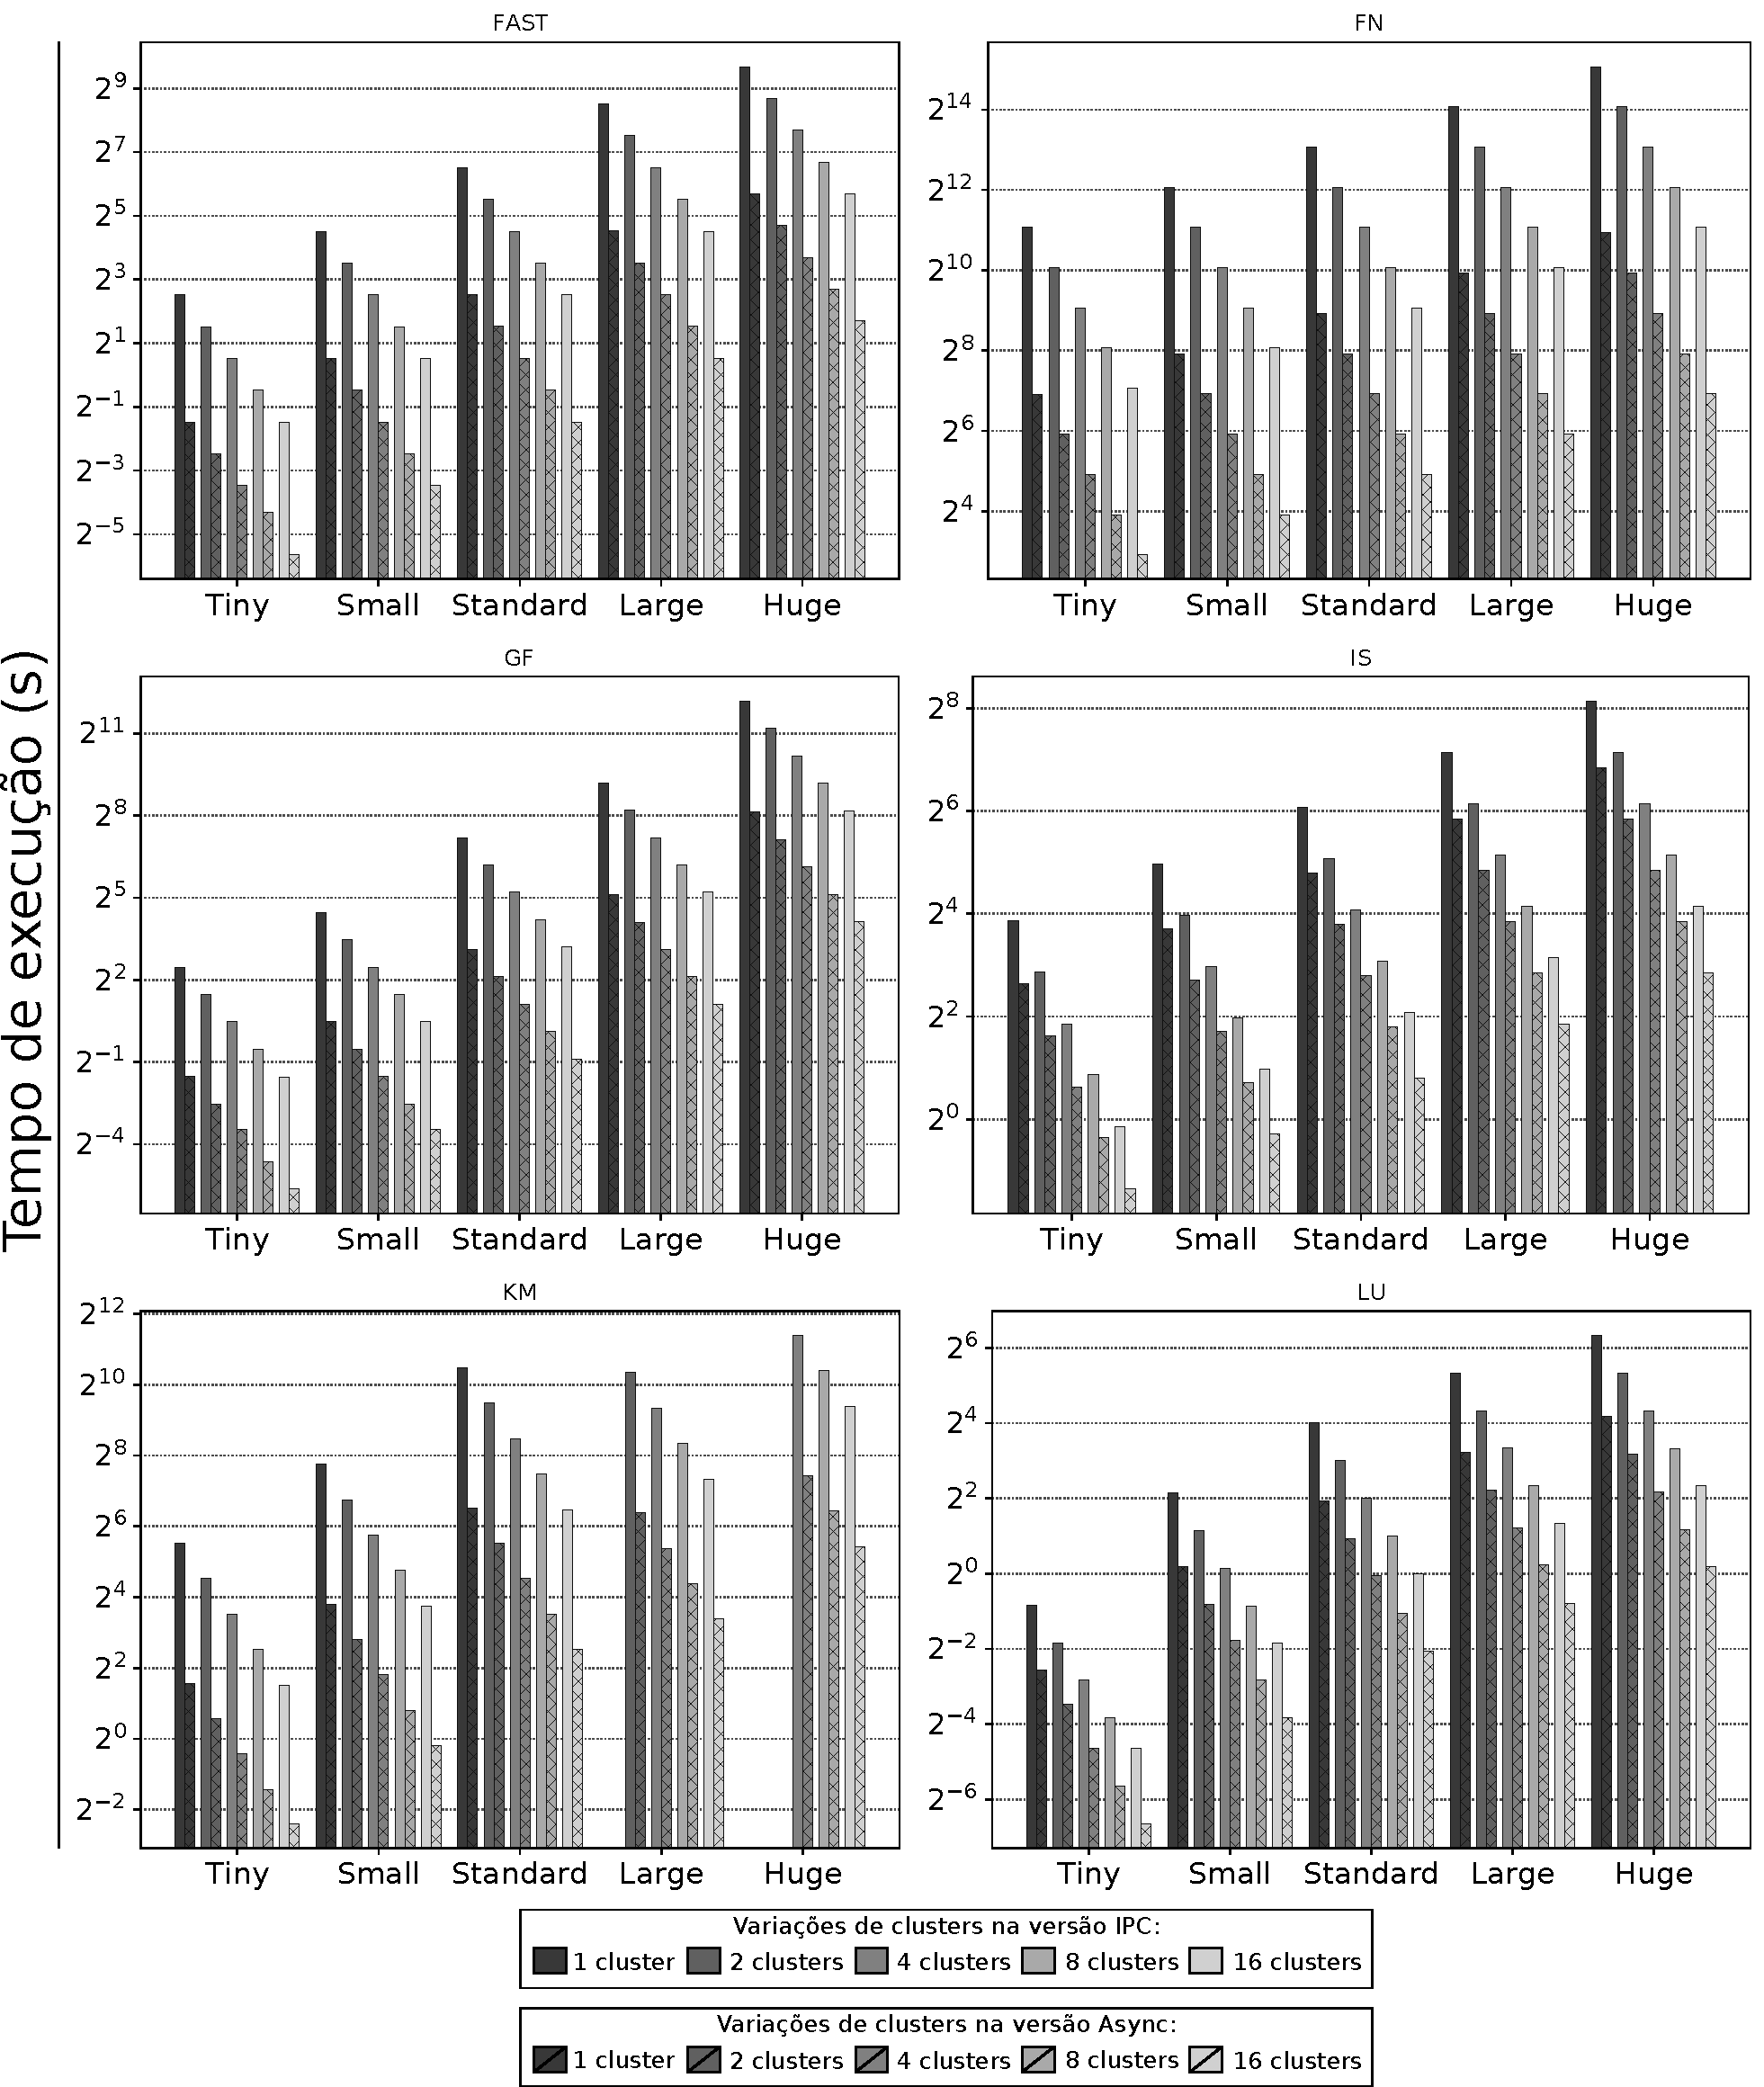
\includegraphics[width=.9\linewidth, keepaspectratio]{slave_time.pdf}
\end{figure}

\begin{figure}[h]
  \centering
  \caption{Tempos de execução do processo \master para cada aplicação.}
  \label{fig:mastertime}
  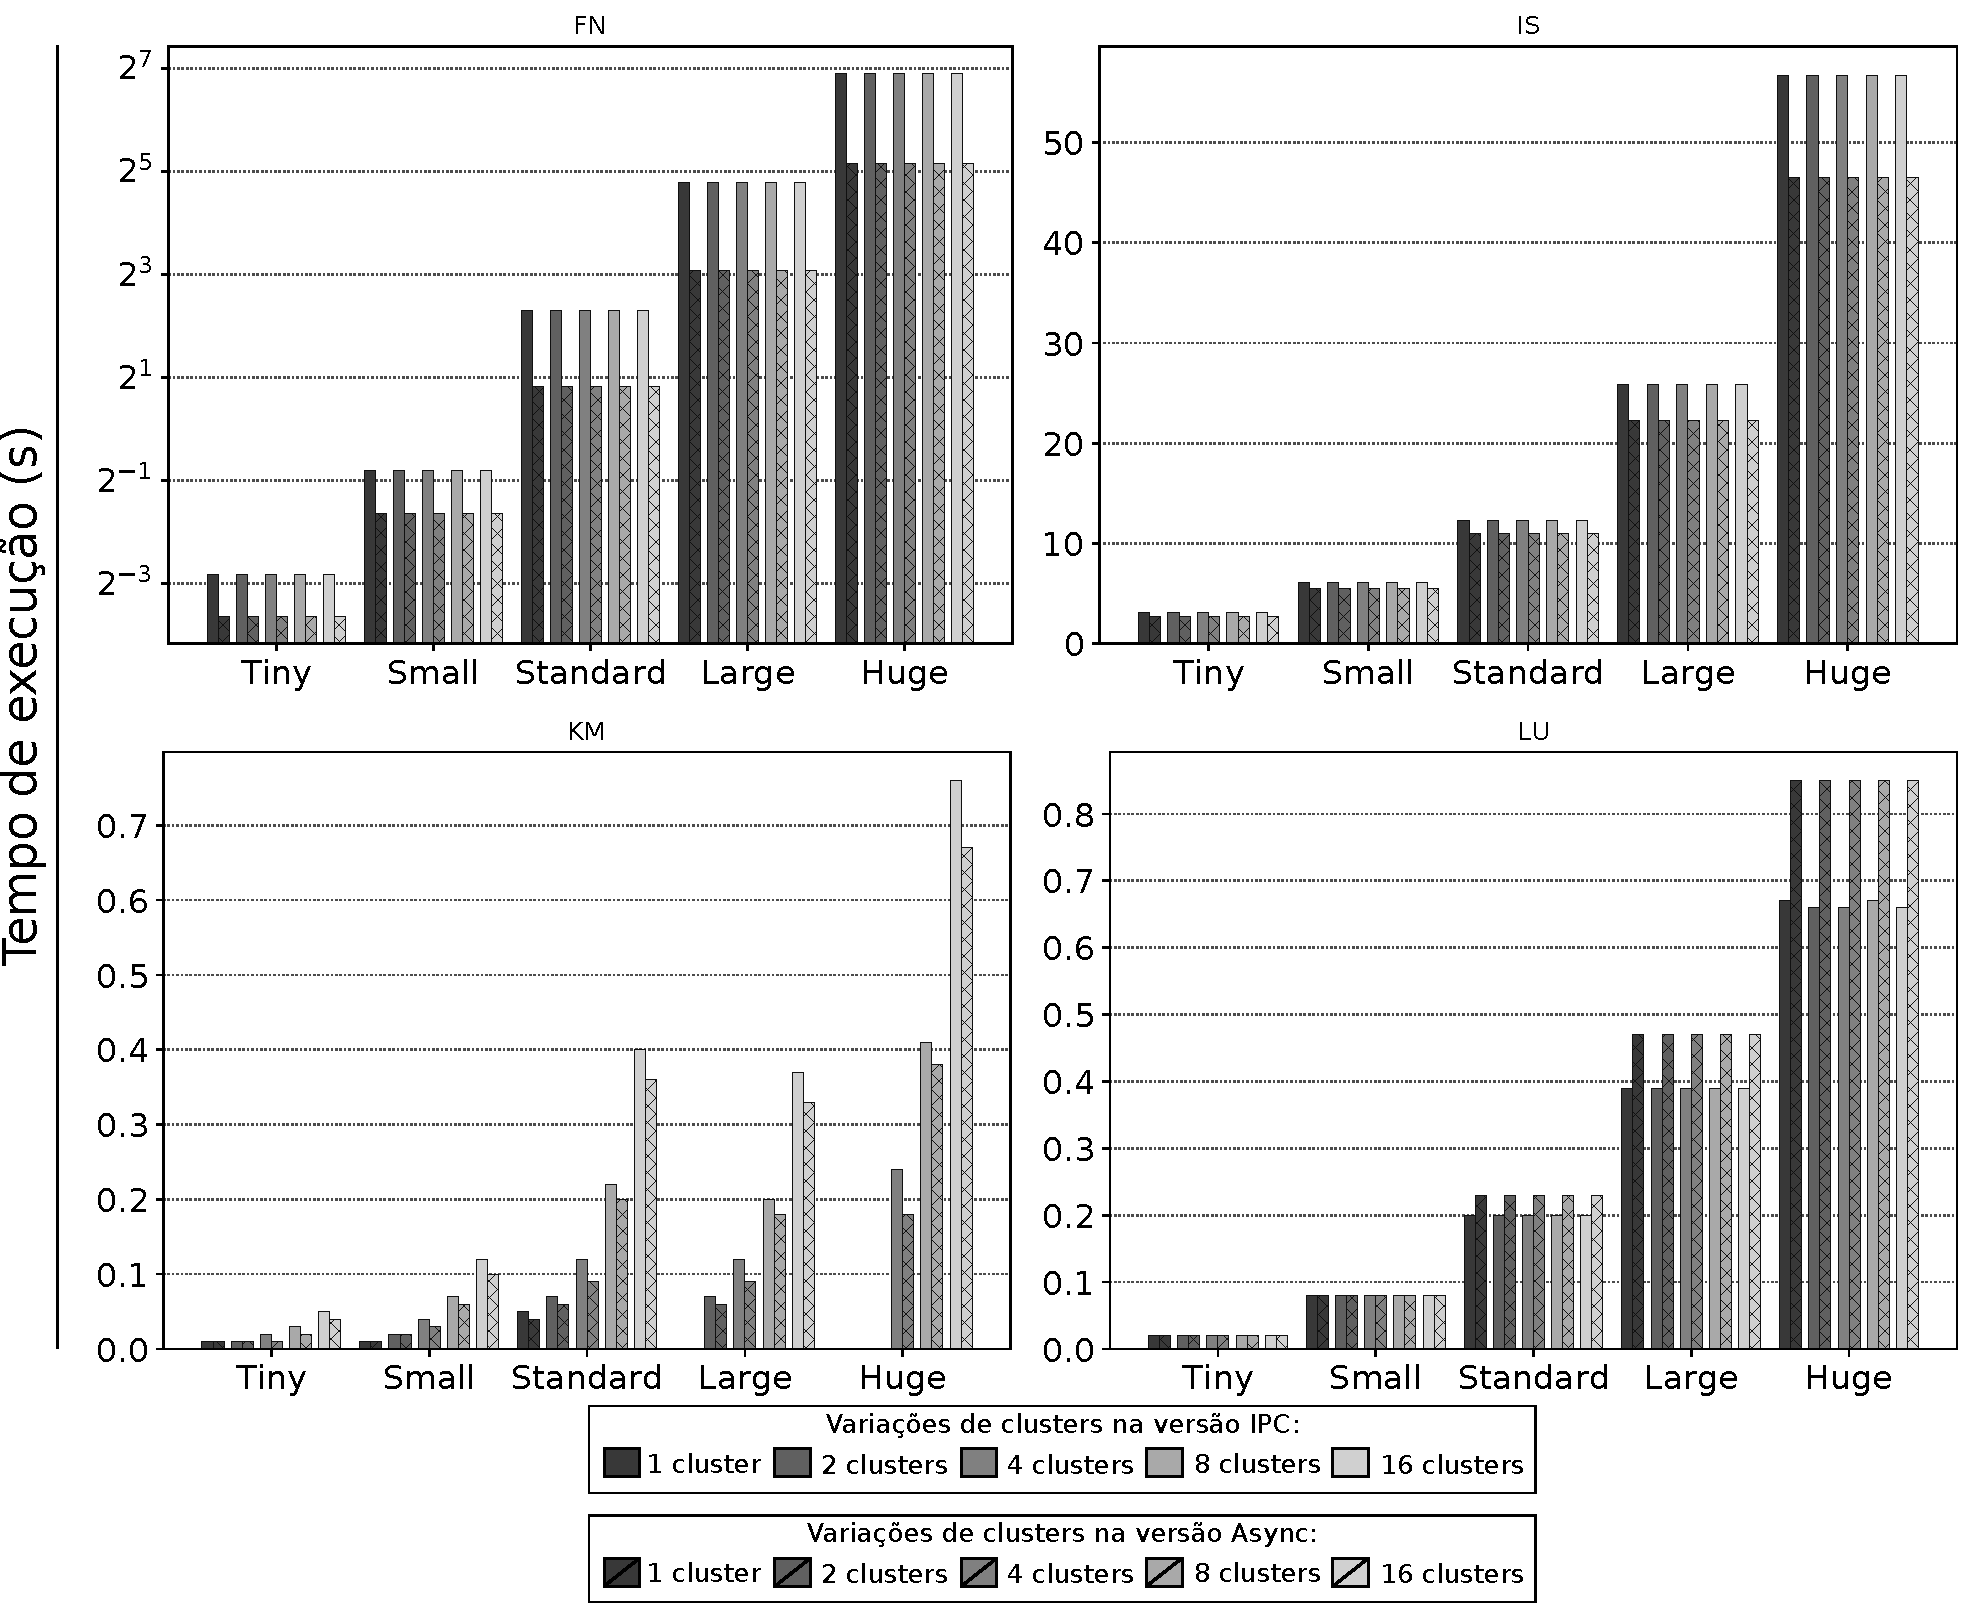
\includegraphics[width=.9\linewidth, keepaspectratio]{master_time.pdf}
\end{figure}

\begin{figure}[h]
  \centering
  \caption{Tempos de comunicação para cada aplicação.}
  \label{fig:commtime}
  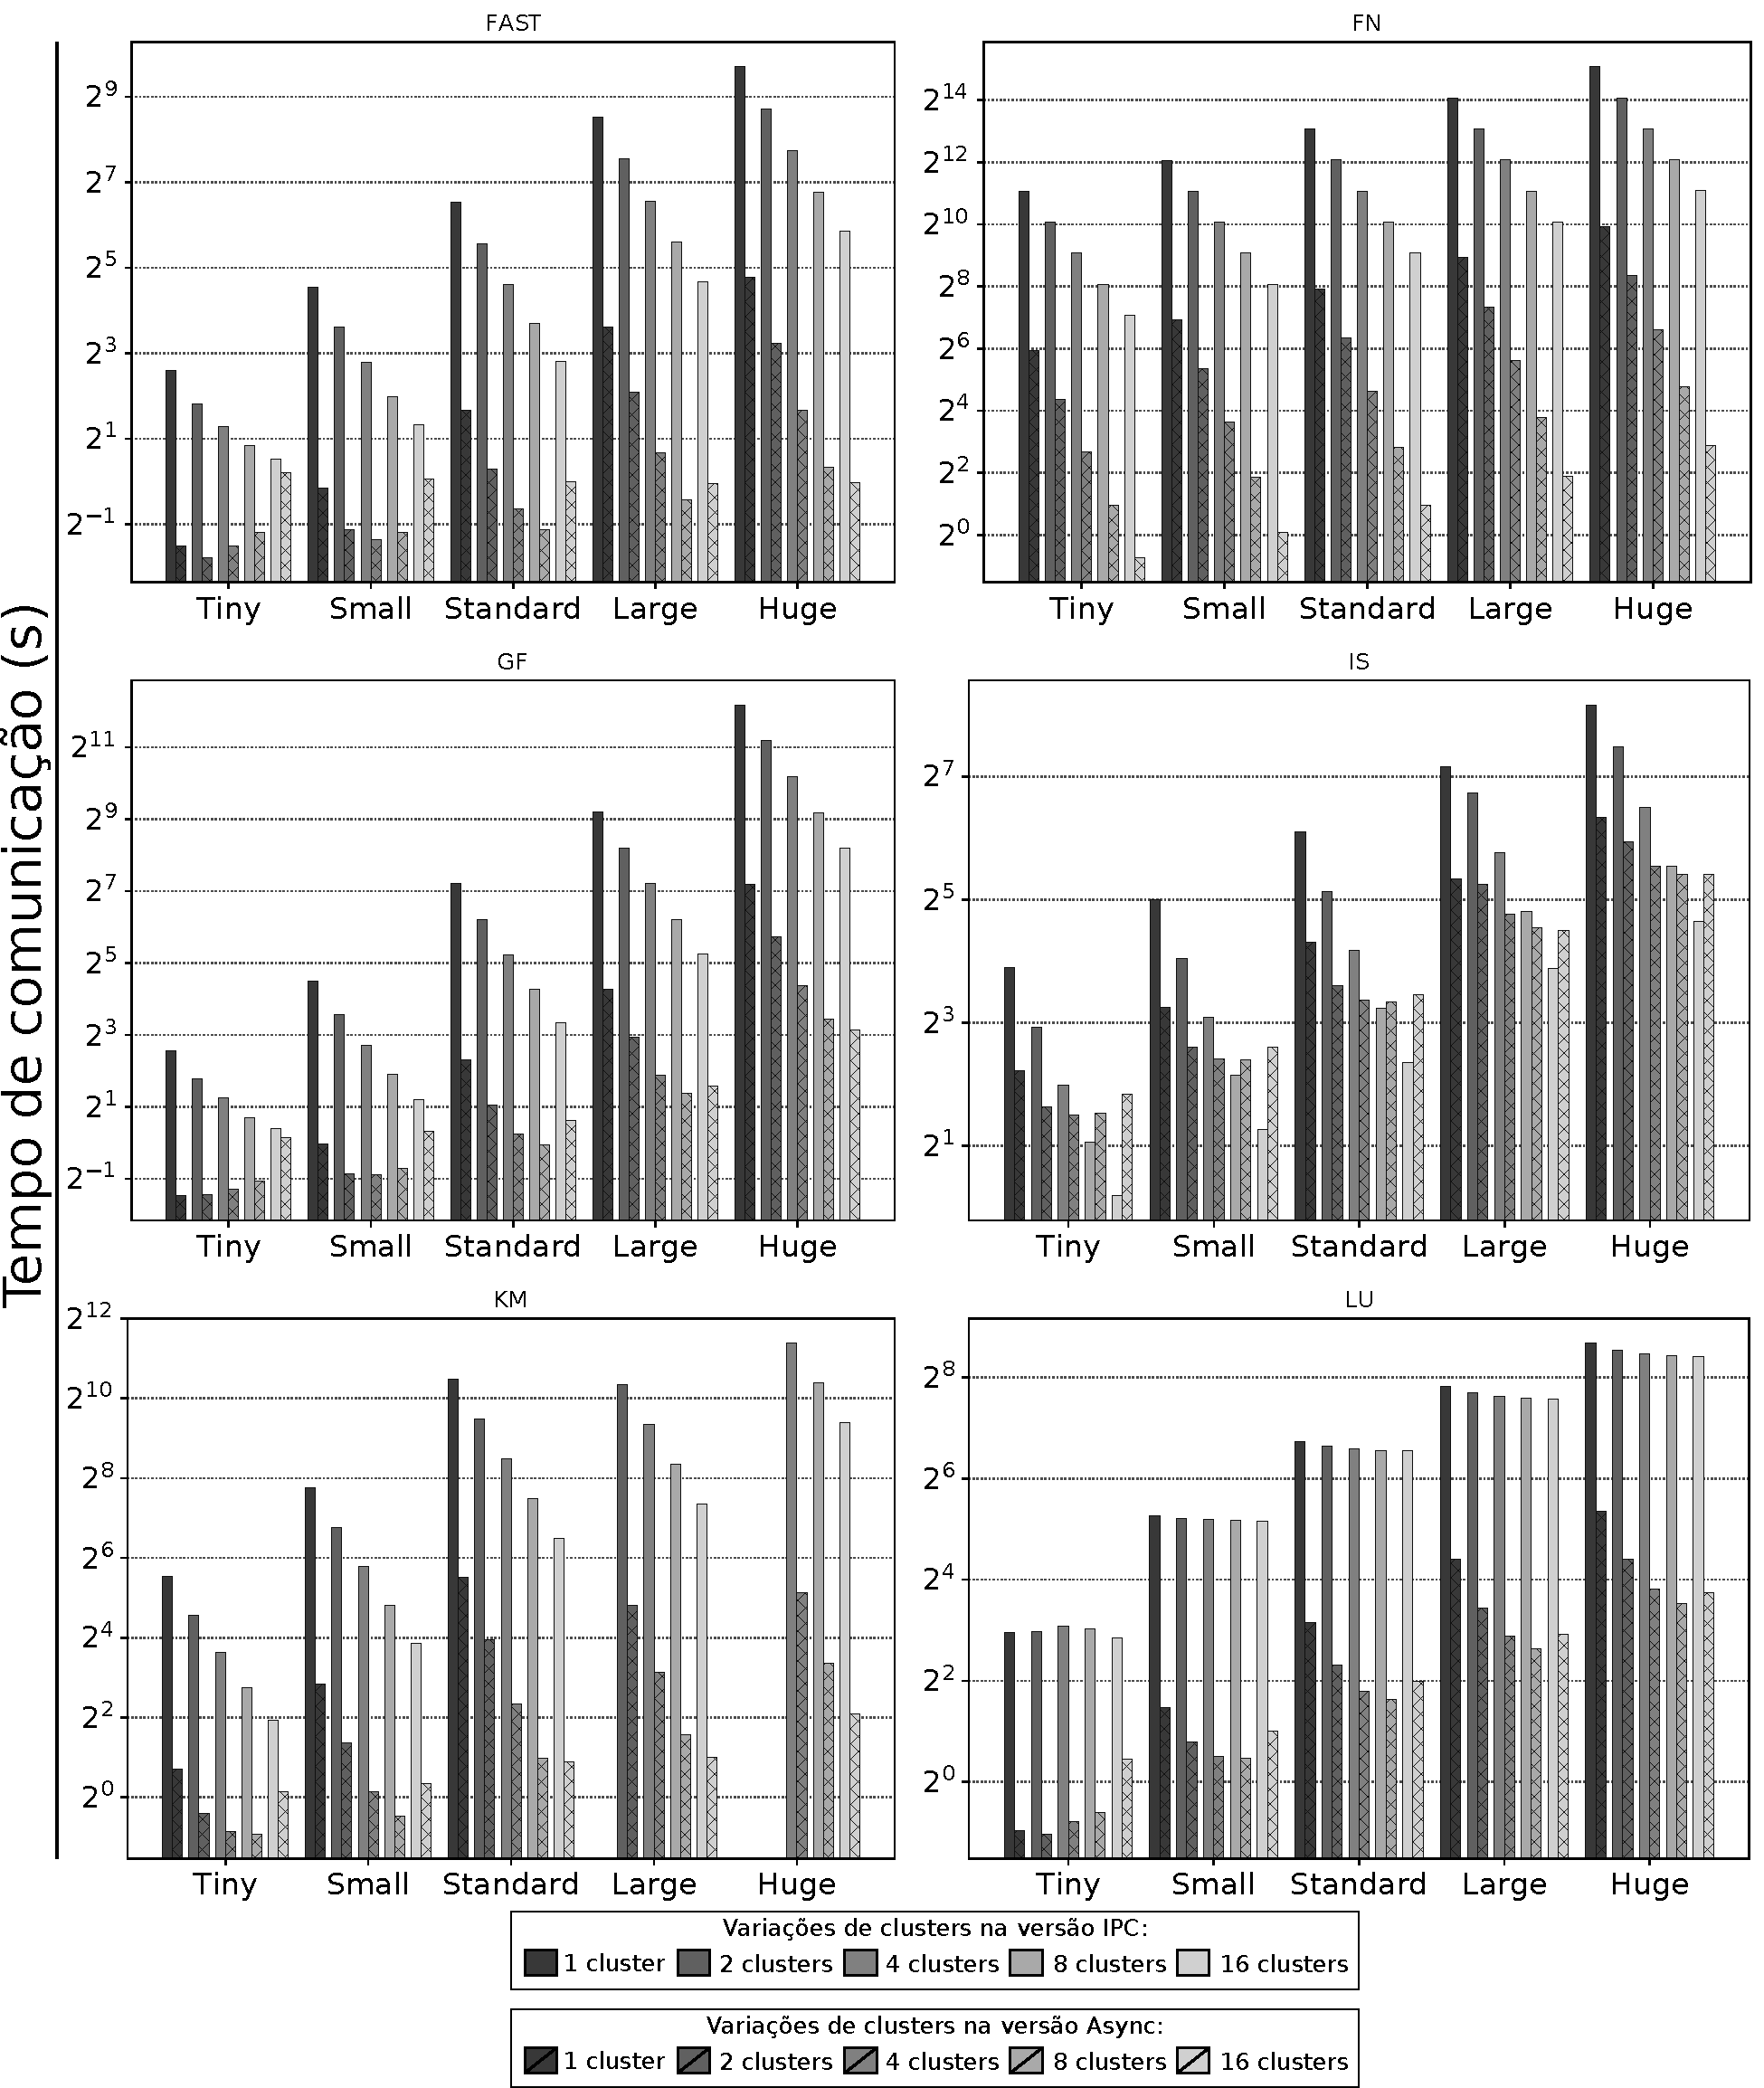
\includegraphics[width=.9\linewidth, keepaspectratio]{comm_time.pdf}
\end{figure}

\section{Análise do Resultado das Métricas de Envio e Recebimento de Dados}
\label{sec:metricasdados}

\begin{table}[h]
\centering
\caption{Reduções ao comparar-se a quantidade de dados que o processo \master envia.}
\label{tab:datasenttable}
\scalebox{0.6}{
\begin{tabular}{l c c c c c c c c c l}
App & \multicolumn{5}{c}{Redução Mínima} & \multicolumn{5}{c}{Reduçã Máxima}

\\\cmidrule(lr){2-6}\cmidrule(lr){7-11}

& Classe & NClusters & IPC(MB) & ASYNC(MB) & Redução(\%) & Classe & NClusters & IPC(MB) & ASYNC(MB) & Redução(\%)\\\midrule

FAST & Tiny & 1 & 4.18 & 4.0 & 4.31 & Huge & 1 & 899.93 & 576.0 & 36.0 \\
FN & Tiny & 1 & 0.05 & 0.05 & 0.0 & Tiny & 2 & 0.05 & 0.05 & 0.0 \\ 
GF & Tiny & 1 & 4.09 & 4.0 & 2.2 & Huge & 16 & 1080.81 & 1024.0 & 5.26 \\
IS & Tiny & 1 & 32.0 & 32.0 & 0.0 & Tiny & 2 & 32.0 & 32.0 & 0.0 \\ 
KM & Small & 8 & 5.53 & 5.88 & -6.33 & Large & 2 & 5.88 & 6.23 & -5.95 \\ 
LU & Large & 1 & 1102.09 & 2730.66 & -147.77 & Huge & 1 & 1494.77 & 853.33 & 42.91 \\

\bottomrule
\end{tabular}}
\end{table}

\begin{table}[h]
\centering
\caption{Reduções ao comparar-se a quantidade de dados que o processo \master recebe.}
\label{tab:datareceivedtable}
\scalebox{0.6}{
\begin{tabular}{l c c c c c c c c c l}
App & \multicolumn{5}{c}{Redução Mínima} & \multicolumn{5}{c}{Reduçã Máxima}

\\\cmidrule(lr){2-6}\cmidrule(lr){7-11}

& Classe & NClusters & IPC(MB) & ASYNC(MB) & Redução(\%) & Classe & NClusters & IPC(MB) & ASYNC(MB) & Redução(\%)\\\midrule

FAST & Huge & 1 & 576.0 & 899.93 & -56.24 & Tiny & 2 & 4.0 & 4.18 & -4.5 \\ 
FN & Tiny & 1 & 0.05 & 0.05 & 0.0 & Tiny & 2 & 0.05 & 0.05 & 0.0 \\
GF & Huge & 16 & 1024.0 & 1080.79 & -5.55 & Small & 1 & 16.0 & 16.38 & -2.37 \\ 
IS & Tiny & 1 & 32.0 & 32.01 & -0.03 & Huge & 1 & 512.0 & 512.03 & -0.01 \\
KM & Tiny & 1 & 0.3 & 0.83 & -176.67 & Standard & 16 & 35.13 & 69.19 & -96.95 \\ 
LU & Large & 1 & 1365.34 & 2996.33 & -119.46 & Tiny & 2 & 170.67 & 171.98 & -0.77 \\

\bottomrule
\end{tabular}}
\end{table}

\begin{figure}[h]
  \centering
  \caption{Quantidade de dados que o processo \master envia aos \slaves.}
  \label{fig:datasent}
  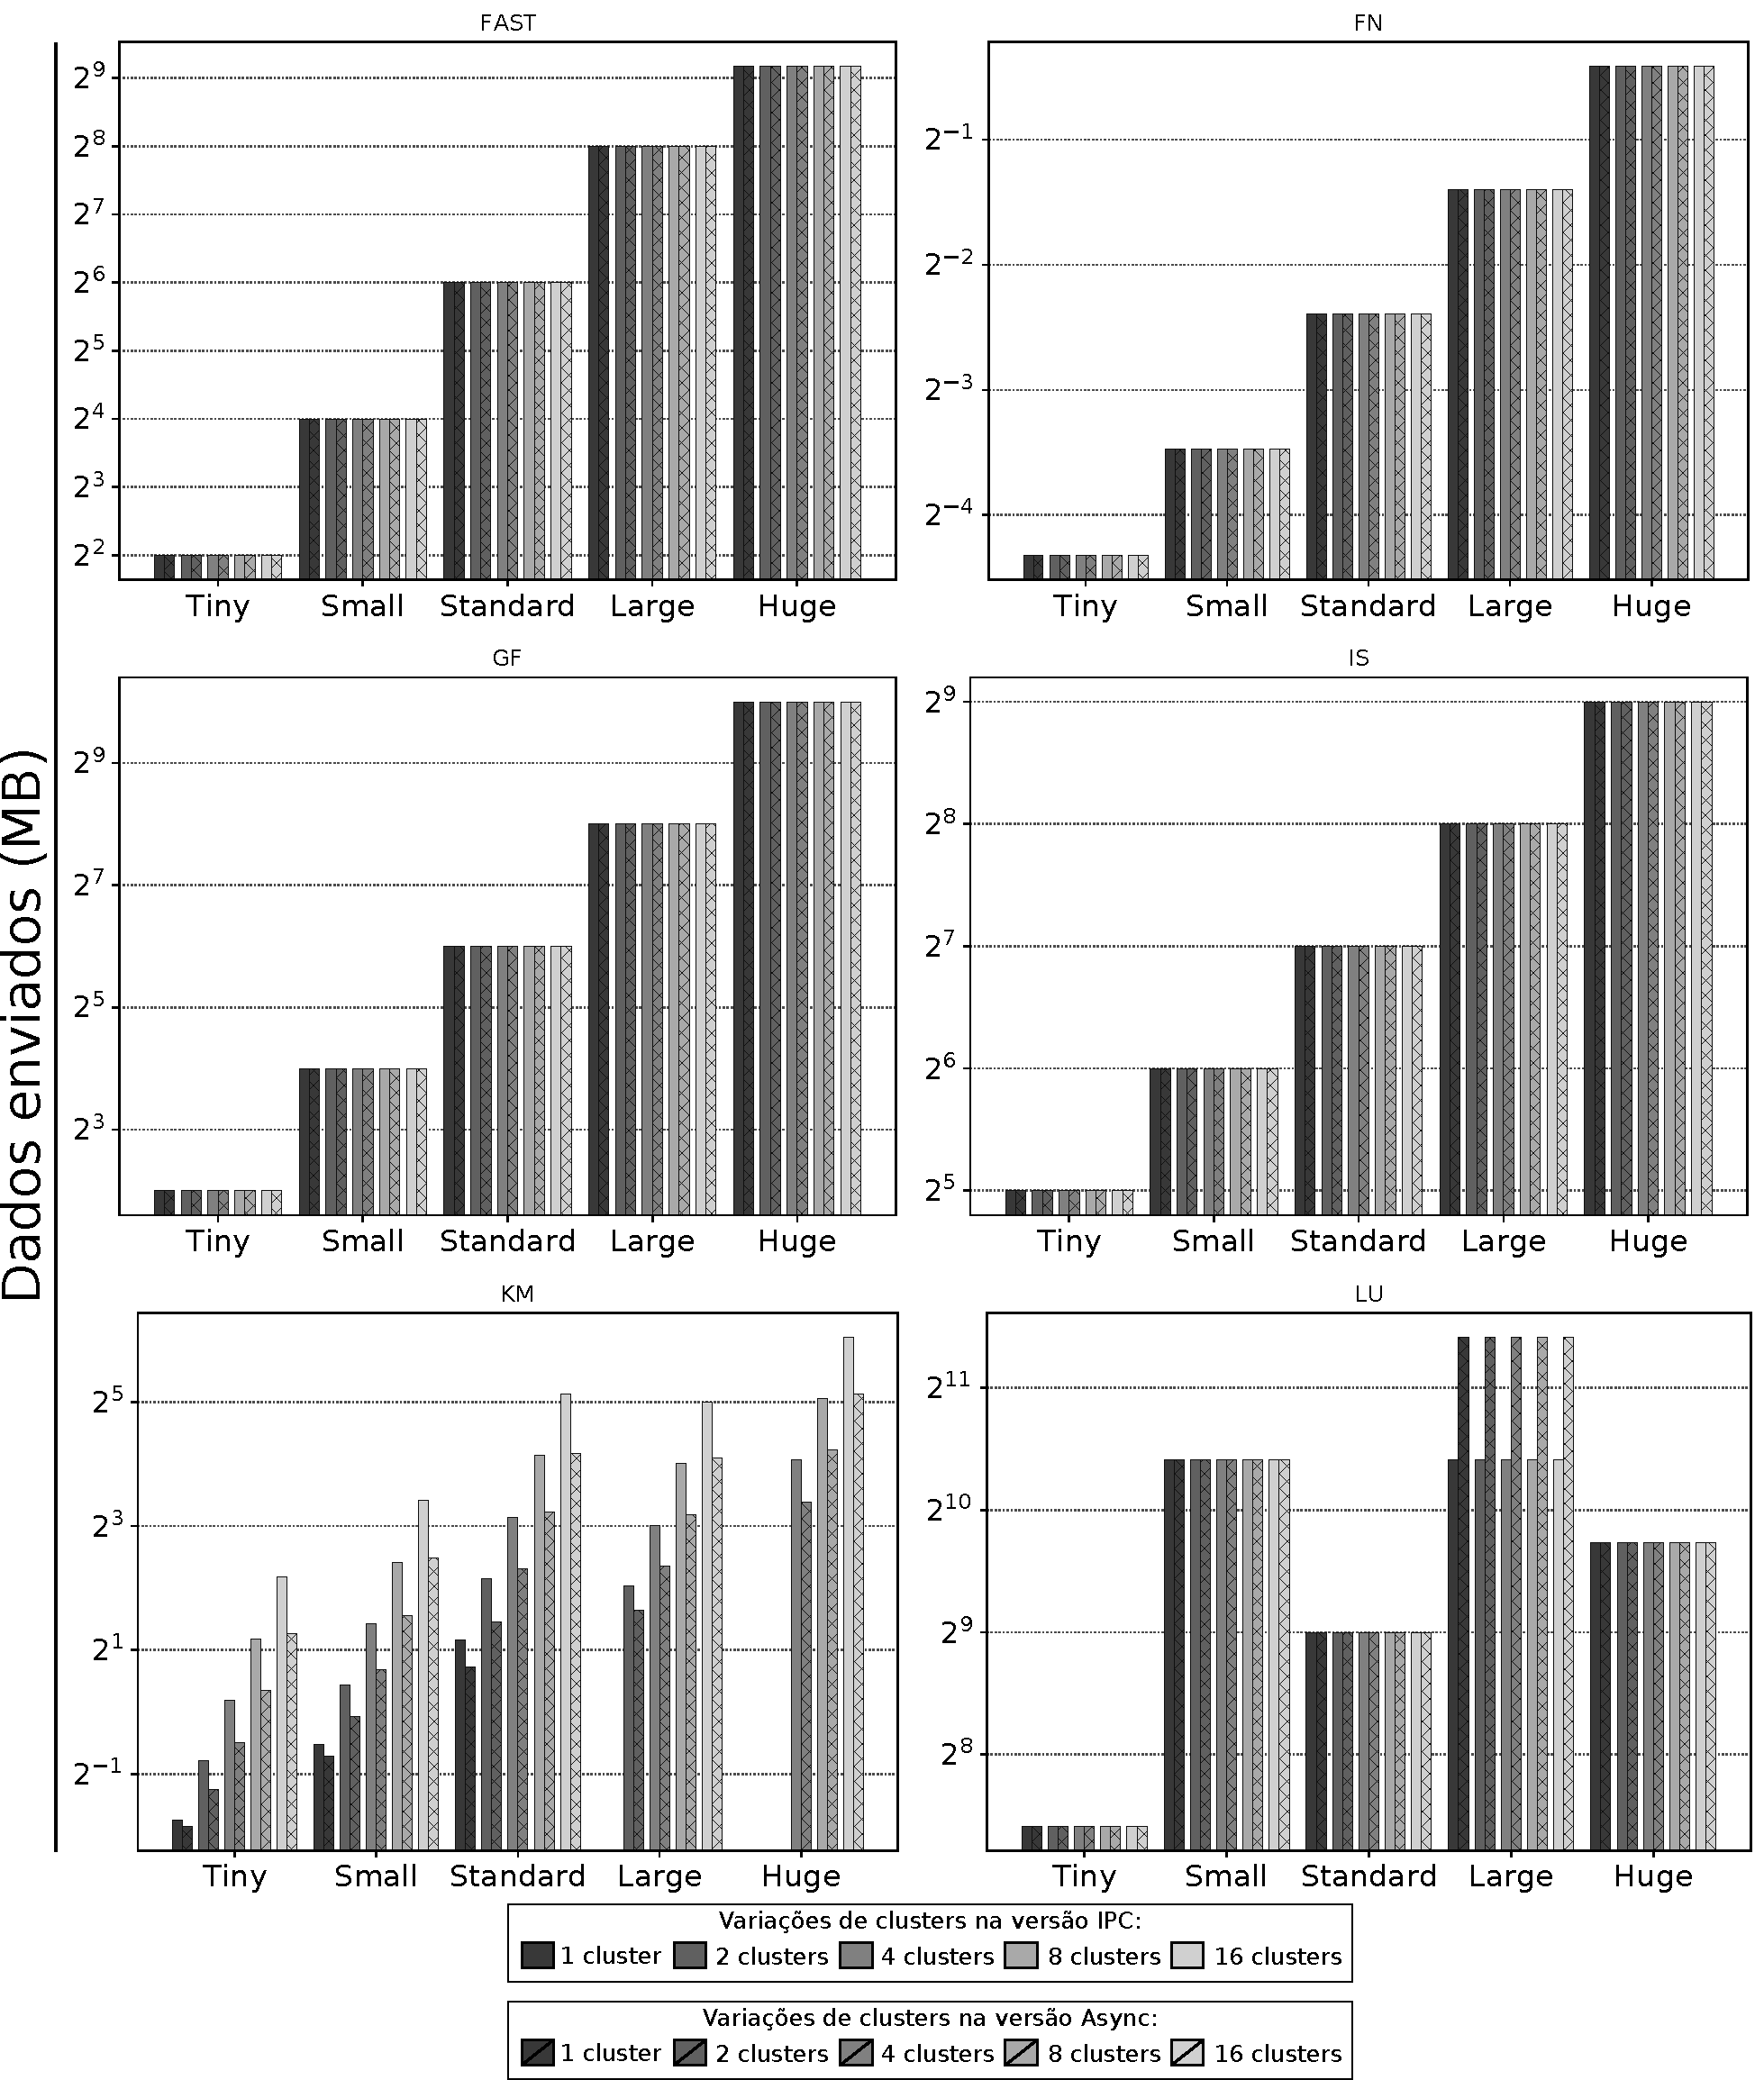
\includegraphics[width=.9\linewidth, keepaspectratio]{data_sent.pdf}
\end{figure}

\begin{figure}[h]
  \centering
  \caption{Quantidade de dados que o processo \master recebe dos \slaves.}
  \label{fig:datareceived}
  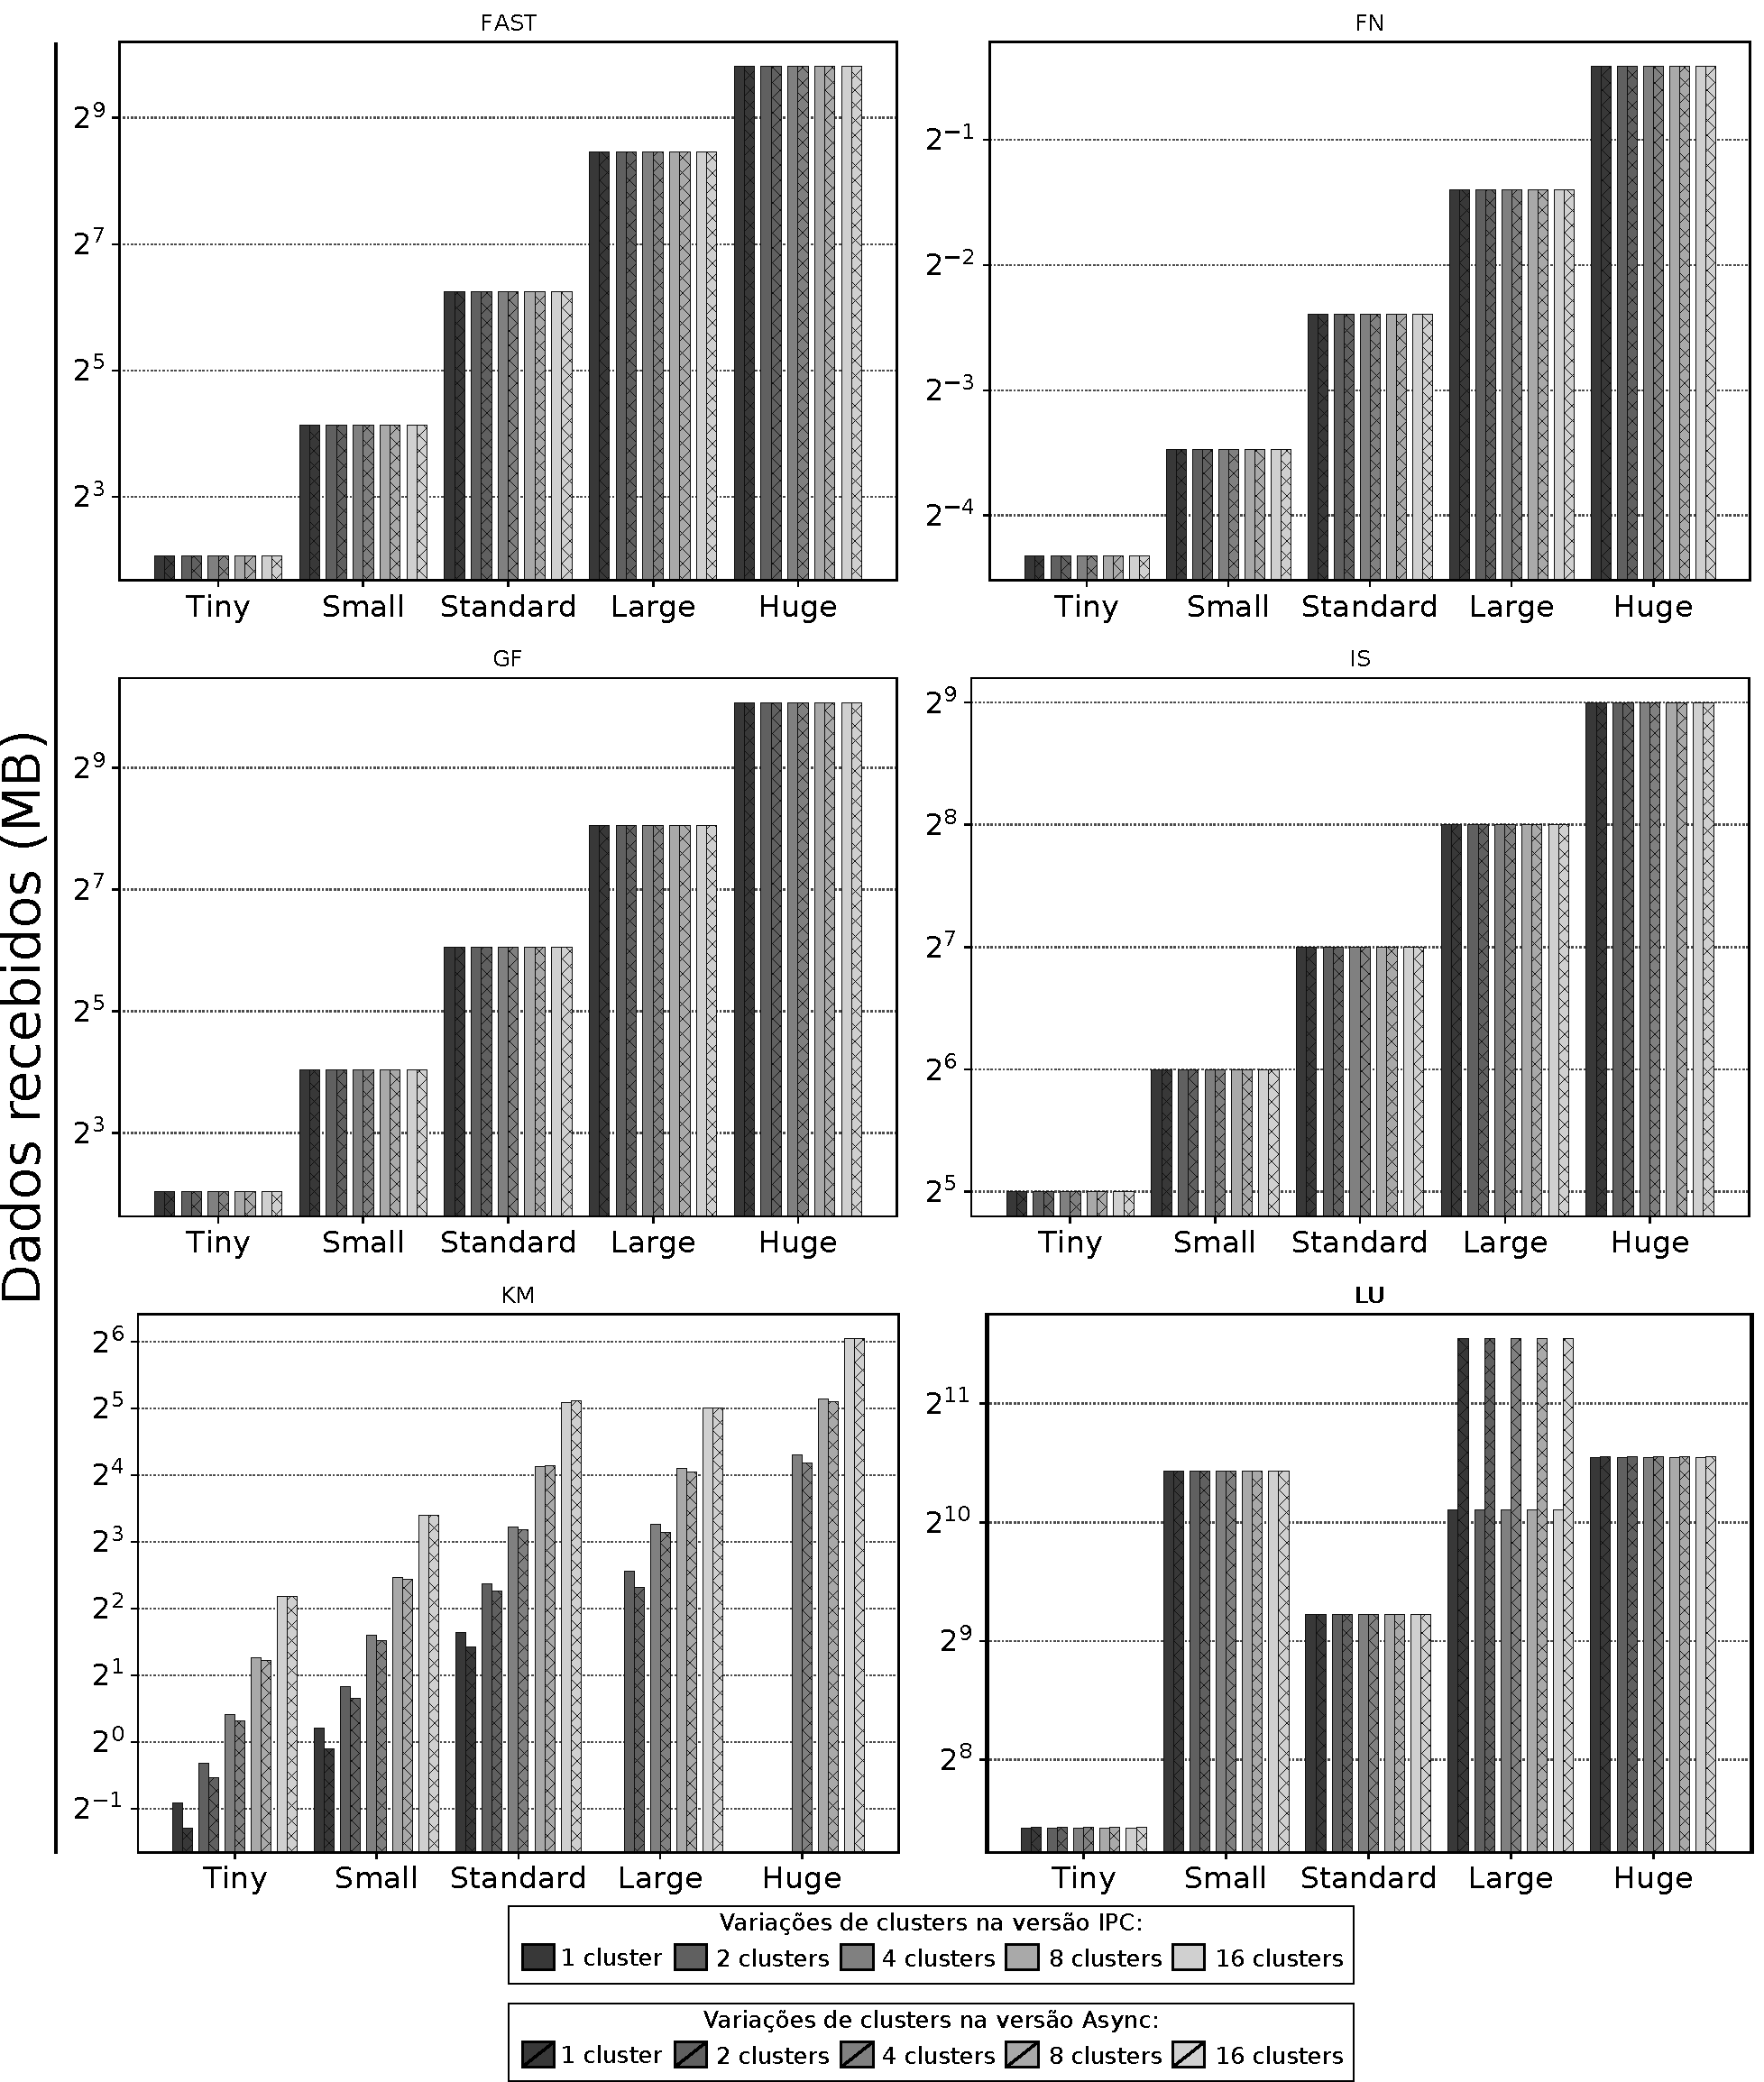
\includegraphics[width=.9\linewidth, keepaspectratio]{data_received.pdf}
\end{figure}

\section{Análise do Resultado das Métricas de Energia}
\label{sec:metricasenergia}

\begin{table}[h]
\centering
\caption{Reduções ao comparar-se a potência média durante execução.}
\label{tab:datareceivedtable}
\scalebox{0.6}{
\begin{tabular}{l c c c c c c c c c l}
App & \multicolumn{5}{c}{Redução Mínima} & \multicolumn{5}{c}{Reduçã Máxima}

\\\cmidrule(lr){2-6}\cmidrule(lr){7-11}

& Classe & NClusters & IPC(W) & ASYNC(W) & Redução(\%) & Classe & NClusters & IPC(W) & ASYNC(W) & Redução(\%)\\\midrule

FAST & Small & 16 & 4.52 & 5.14 & -13.72 & Small & 1 & 4.27 & 4.11 & 3.75 \\
FN & Large & 16 & 4.79 & 10.25 & -113.99 & Huge & 1 & 4.28 & 4.76 & -11.21 \\
GF & Huge & 16 & 4.84 & 5.91 & -22.11 & Small & 1 & 4.27 & 4.17 & 2.34 \\
IS & Large & 16 & 4.48 & 5.99 & -33.71 & Large & 1 & 4.28 & 4.41 & -3.04 \\
KM & Huge & 16 & 4.82 & 11.21 & -132.57 & Small & 1 & 4.25 & 4.71 & -10.82 \\
LU & Huge & 16 & 4.42 & 6.05 & -36.88 & Small & 1 & 4.23 & 4.09 & 3.31 \\

\bottomrule
\end{tabular}}
\end{table}

\begin{table}[h]
\centering
\caption{Reduções ao comparar-se o gasto energético total.}
\label{tab:datareceivedtable}
\scalebox{0.6}{
\begin{tabular}{l c c c c c c c c c l}
App & \multicolumn{5}{c}{Redução Mínima} & \multicolumn{5}{c}{Reduçã Máxima}

\\\cmidrule(lr){2-6}\cmidrule(lr){7-11}

& Classe & NClusters & IPC(J) & ASYNC(J) & Redução(\%) & Classe & NClusters & IPC(J) & ASYNC(J) & Redução(\%)\\\midrule

FAST & Tiny & 16 & 38.79 & 43.92 & -13.23 & Huge & 1 & 3759.55 & 456.35 & 87.86 \\
FN & Tiny & 16 & 666.97 & 129.65 & 80.56 & Standard & 1 & 36549.92 & 2325.1 & 93.64 \\
GF & Tiny & 16 & 38.4 & 44.64 & -16.25 & Huge & 1 & 20504.65 & 1783.83 & 91.3 \\
IS & Tiny & 16 & 52.2 & 68.02 & -30.31 & Large & 1 & 751.9 & 395.02 & 47.46 \\
KM & Tiny & 16 & 47.55 & 46.21 & 2.82 & Standard & 1 & 6131.17 & 460.56 & 92.49 \\
LU & Tiny & 16 & 64.68 & 44.14 & 31.76 & Huge & 8 & 1535.77 & 103.8 & 93.24 \\

\bottomrule
\end{tabular}}
\end{table}

\begin{figure}[h]
  \centering
  \caption{Potência média durante a execução de cada aplicação.}
  \label{fig:avgpower}
  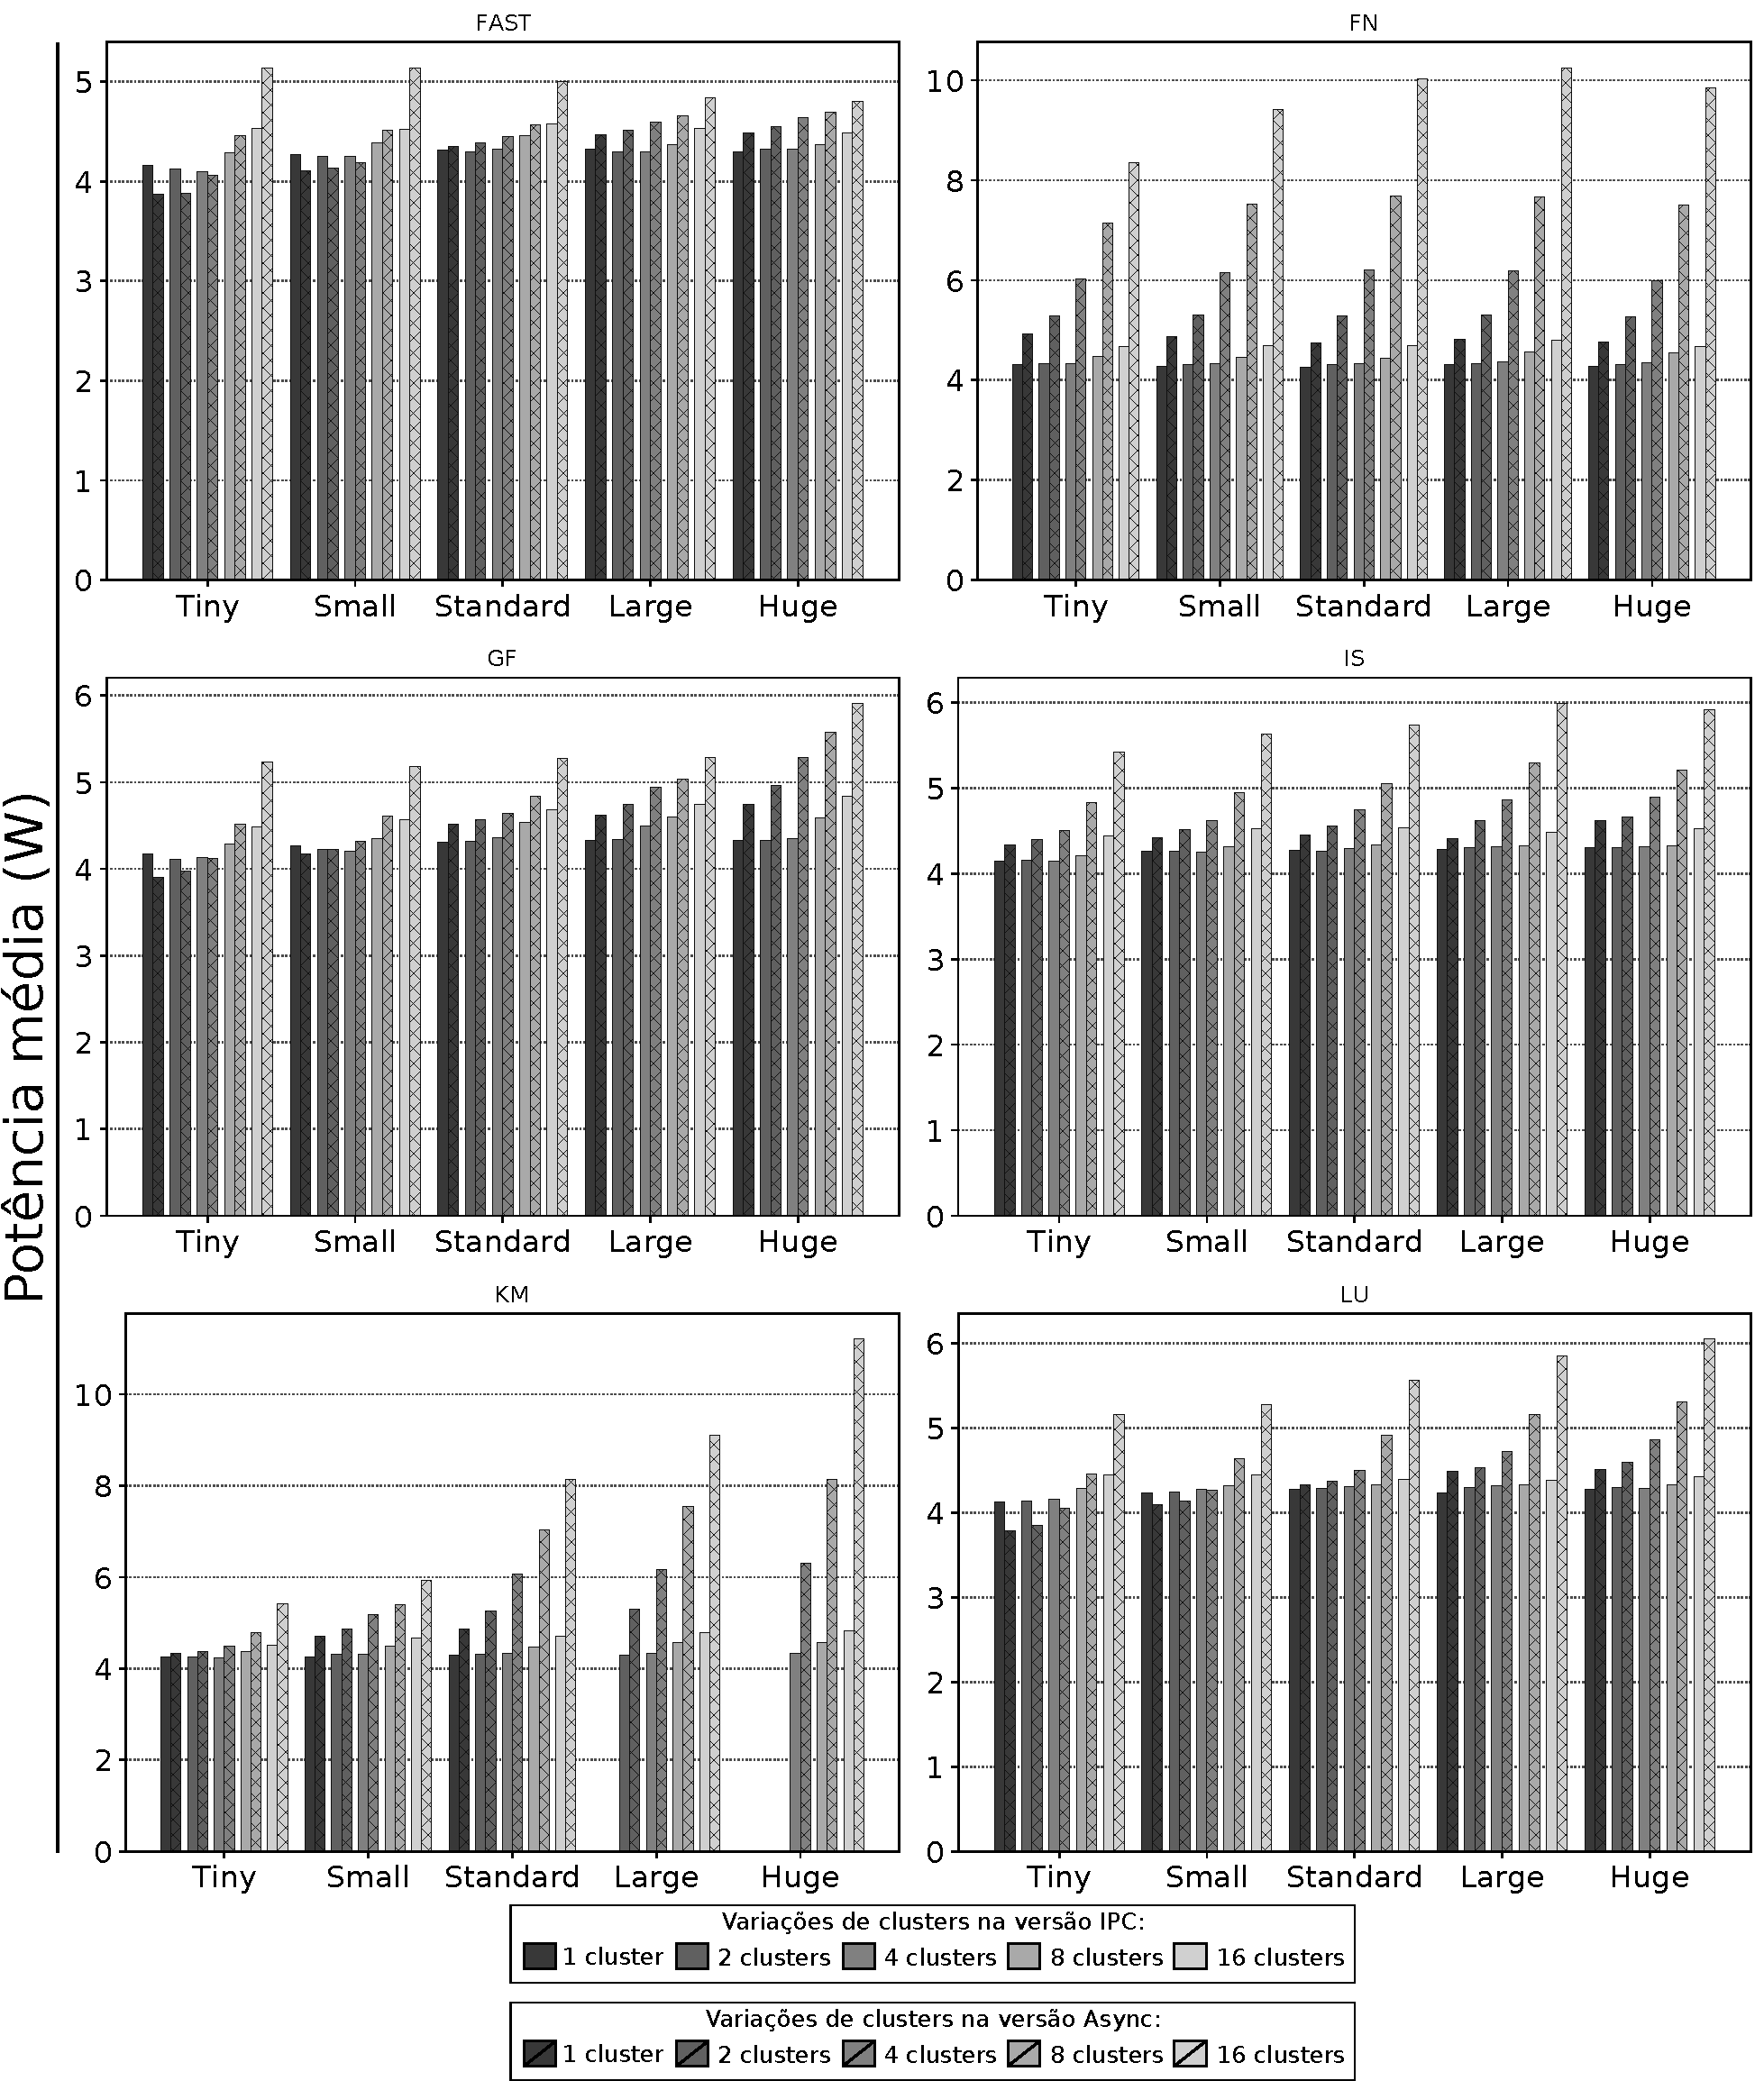
\includegraphics[width=.9\linewidth, keepaspectratio]{avg_power.pdf}
\end{figure}

\begin{figure}[h]
  \centering
  \caption{Gasto energético de cada aplicação.}
  \label{fig:energy}
  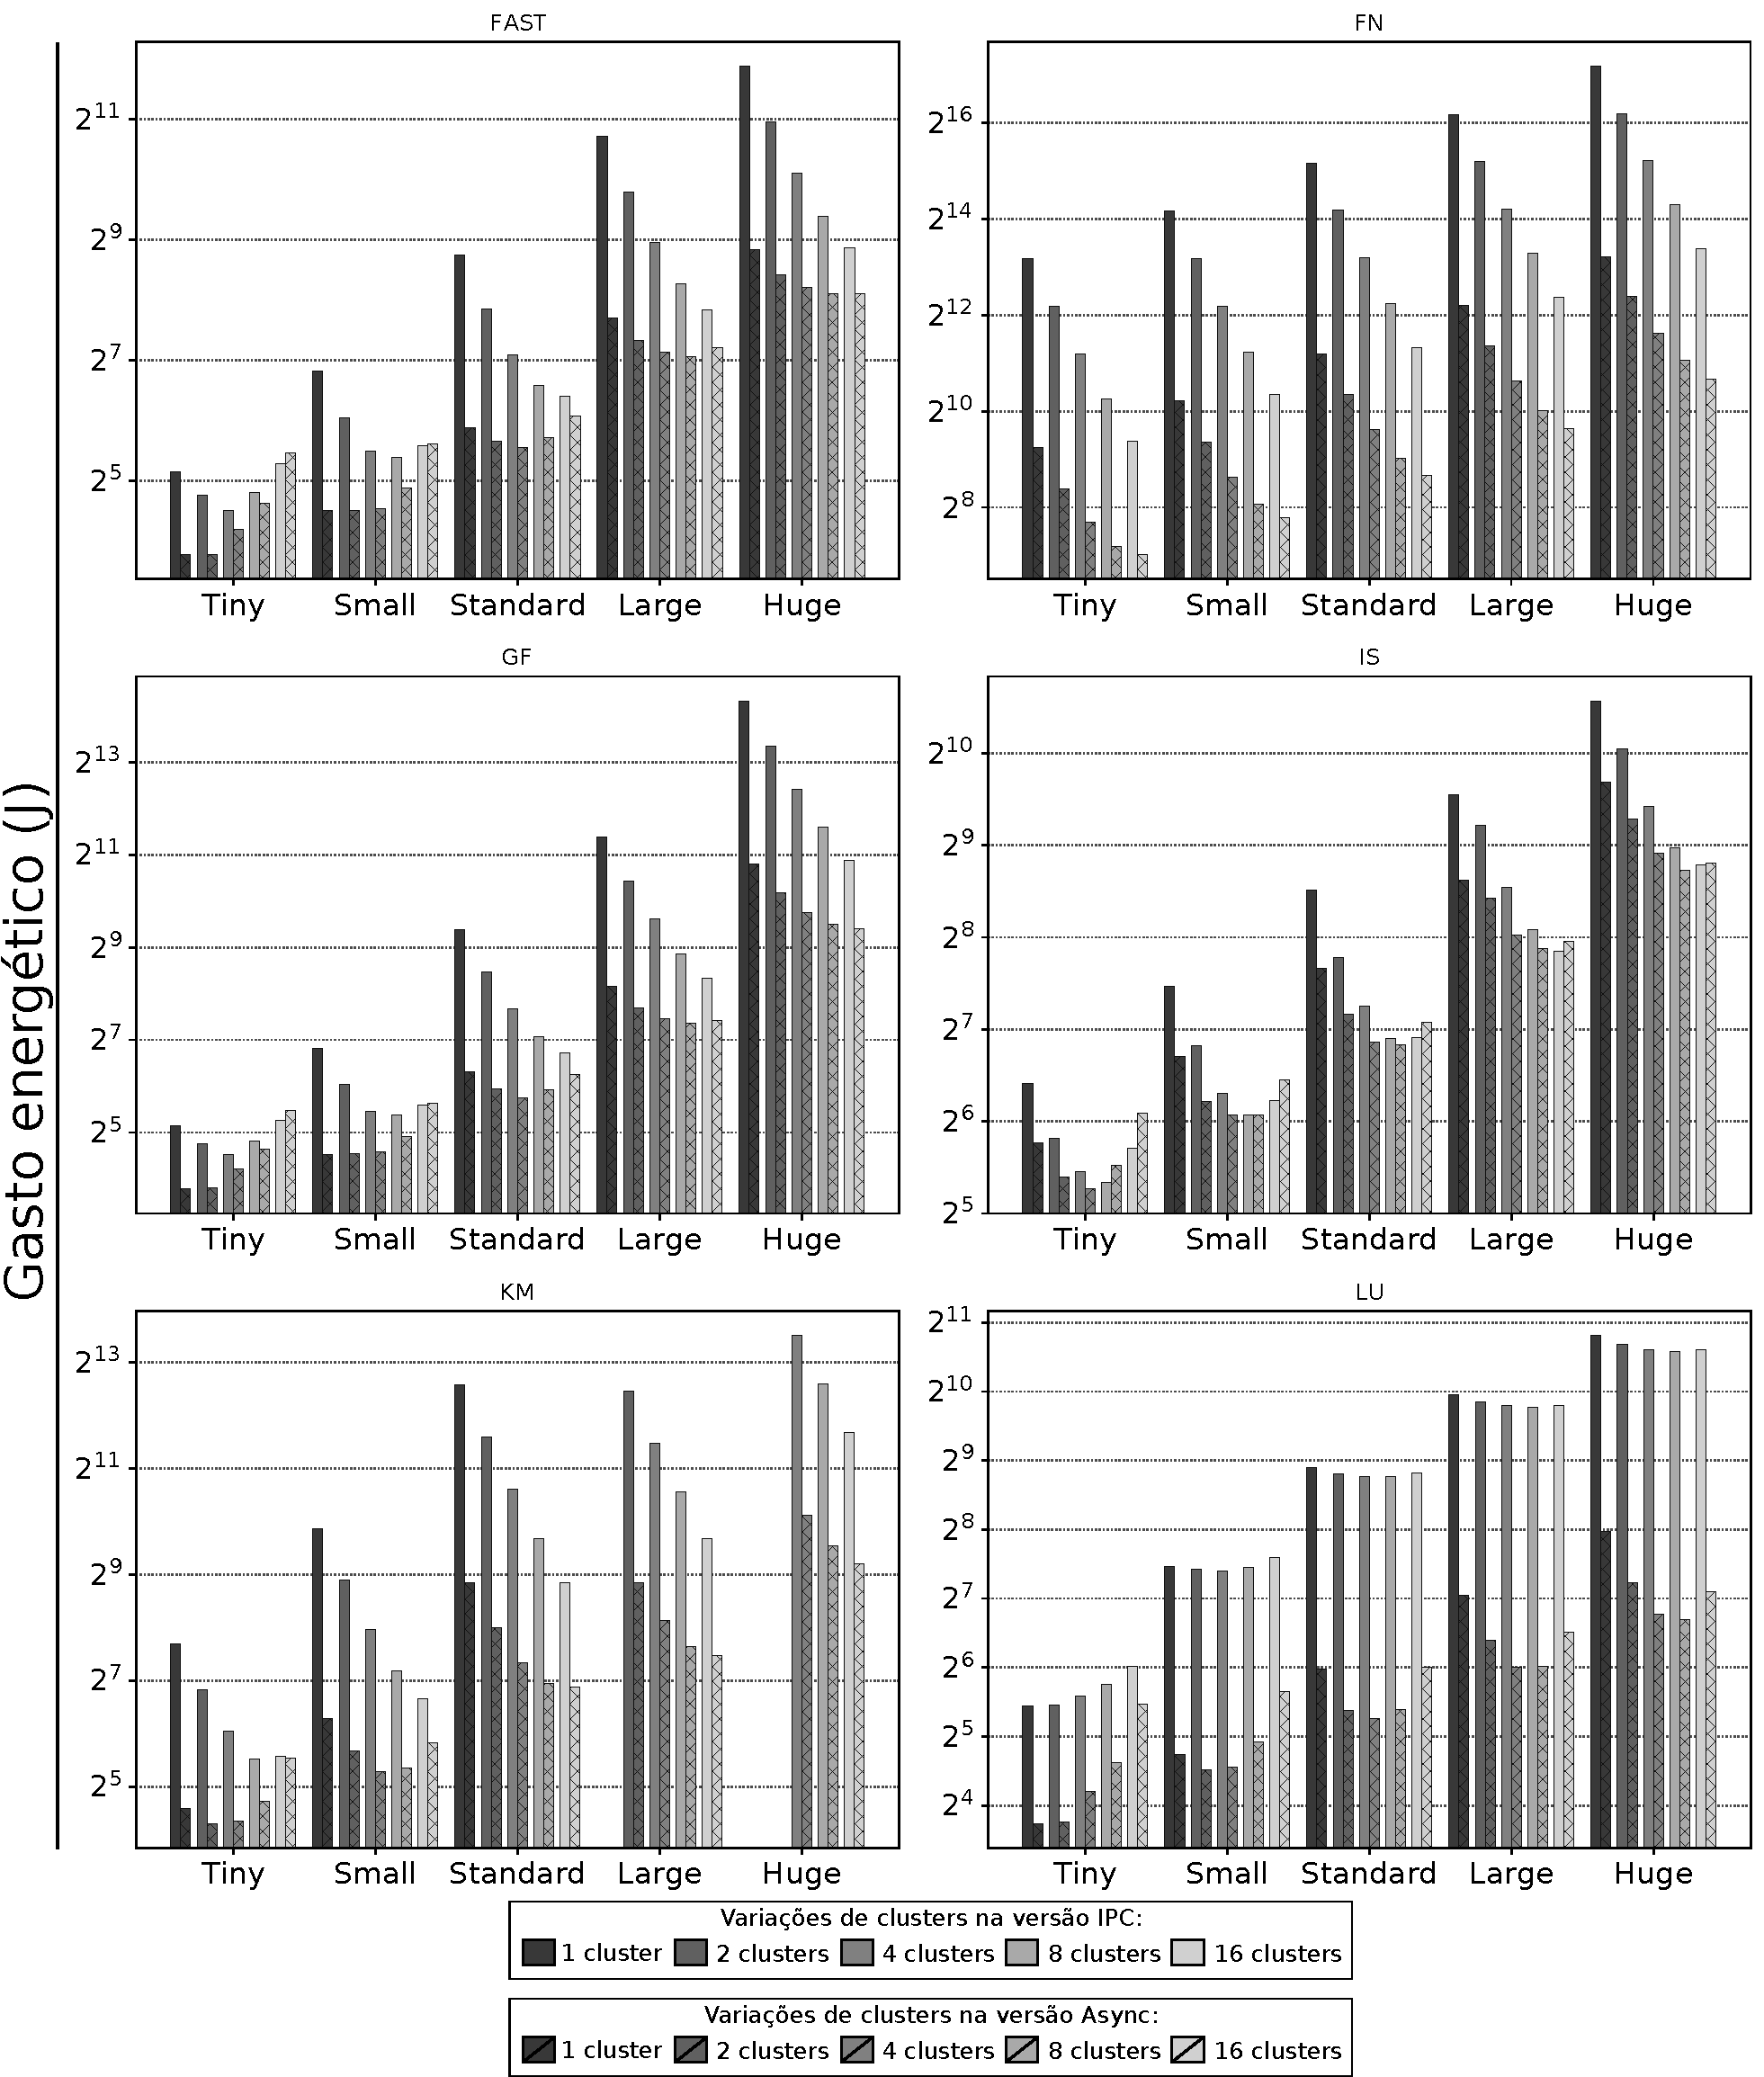
\includegraphics[width=.9\linewidth, keepaspectratio]{energy.pdf}
\end{figure}


\chapter{Conclusão}
\label{ch:conclusao}

\index{bobagem} Primeiro parágrafo da seção com uma frase sem sentido que só serve para ocasionar uma quebra e de demonstrar a configuração de indentação da primeira linha. Essa frase está aqui pois parágrafos de uma linha são feios.

Resultado do uso de siglas:
\begin{itemize}
\item Sigla que nunca expande: \API;
\item Sigla normal, expande no primeiro uso: \DHT, mas não no segundo: \DHT;
\item Siglas com plurais automaticos: \APIs e \DHTs;
\item Plural não-trivial: \SQs;
\item Forçando uma expansão (e no plural) \Glsfirstplural{DHT};
\item Usando uma sigla cujo comando é diferente da sigla: \WTC.
\end{itemize}

Resultado do glossário:
\begin{itemize}
\item Dois termos, \polling e \proxy;
\item Plural: \proxys.
\end{itemize}

Resultado de \mla|index|: primeiro um link normal \indexterm{tomate}, depois um capitalizado \indexTerm{tomate}.

\begin{defn}
  Exemplo de definição
\end{defn}

\begin{theorem}
  Exemplo de teorema
\end{theorem}

\begin{theoremproof}
  Exemplo de prova \qed
\end{theoremproof}

(Sub)enumerações e citações (verificar se OK com o idioma):
\begin{enumerate}
\item \cite{turing1937}:
  \begin{enumerate}
  \item \citeonline{turing1937}:
    \begin{enumerate}
    \item \citeonline{dijkstra1968};
    \end{enumerate}
  \end{enumerate}
\item \cite{turing1937,dijkstra1968};
\item \citeonline{turing1937,dijkstra1968}.
\end{enumerate}


\begin{listing}[tb]
\caption{Meta informações do presente documento.}
\label{lst:meta}
\begin{minted}[highlightlines={1,4-5}]{latex}
\titulo{Template \LaTeX{} para testes e dissertações do LAPESD/UFSC}
\autor{Omar Ravenhurst}
\data{1 de agosto de 2019} % ou \today
\tese % ou \dissertacao
\titulode{Doutor em Ciência da Computação}
\orientador{Prof. Ben Trovato, Dr.}
\coorientador{Prof. Lars Thørväld, Dr.}

\membrobanca{Prof. Valerie Béranger, Dr.}{Universidade Federal de Santa Catarina}
\membrobanca{Prof. Mordecai Malignatus, Dr.}{Universidade Federal de Santa Catarina}
\membrobanca{Prof. Huifen Chan, Dr.}{Universidade Federal de Santa Catarina}
\coordenador{Prof. Charles Palmer, Dr.}
\end{minted}
\fonte{o autor.}
\end{listing}


Resultado de \mla|\autoref|s:
\begin{itemize}
\item \autoref{lst:meta};
\item \autoref{alg:algoritmo};
\item \autoref{fig:figura} tem subfiguras:
  \begin{itemize}
  \item \autoref{fig:svg}
  \item \autoref{fig:brasao}
  \end{itemize}
\item \autoref{tb:tabela};
\item \autoref{ch:exemplo};
\item \autoref{sec:frutas};
\item \autoref{sec:goiaba};
\item \autoref{sec:jabuticaba};
\item \autoref{sec:tomate}.
\end{itemize}


\begin{algorithm}
  \caption{Exemplo do ambiente \texttt{algorithimic}.}
  \label{alg:algoritmo}
  \begin{algorithmic}[1]
    \Procedure{Closure}{C, A}
      \State{$H \gets \emptyset$}\Comment{Direct cache}
      \For{$i \in [1, n]$}\Comment{Parallel, (dynamic,32) scheduling}
        \State{$H \gets H \cup \Call{DoImportantStuff}{i}$}
      \EndFor
    \EndProcedure
  \end{algorithmic}
  \fonte{o autor.}
\end{algorithm}

\begin{figure}[tb]
  \centering
  \caption{Exemplo de figura com duas subfiguras.}   
  \label{fig:figura}
  
  % Subfiguras são feitas usando as funcionalidades do memoir. Não
  % inclua outros pacotes, pois eles podem fazer o memoir dar ragequit
  % 
  % Há duas maneiras, a maneira limpinha (só no lapesd-thesis.cls) e a
  % maneira do memoir (aviso: \subtop não funciona direito).
  \subcaptionminipage[fig:svg]%
    {.49\linewidth}%
    {O Makefile compila SVGs em PDFs usando o inkscape}%
    {
\includegraphics[width=.2\linewidth]{alphachannel.pdf}}%
  \hfill% 
  % o comando acima expande para o equivalente disso:
  \begin{minipage}[t]{.49\linewidth}%
    \centering
    \subcaption{Brasão da UFSC.\label{fig:brasao}}
    \includegraphics[width=.2\linewidth]{\jobname-logo.pdf}
  \end{minipage}

  \fonte{o autor.}
\end{figure}

\begin{table}[tb]
  \centering
  \caption{Exemplo de tabela e símbolos}
  \label{tb:tabela}
  \begin{tabular}{lccp{5cm}}
    \toprule
    Esquerda & Coluna 1    & \rotatebox{90}{90 graus}  & Parágrafo com \mla|p{5cm}|   \\
    \midrule
    $r_1$    & \cmk        &  \xmk                     & \circledi    \\
    $r_2$    &     \multicolumn{2}{c}{merged cell}     & \circledii   \\
    $r_3$    & \circlediii & \circlediv                & \circledv    \\
    $r_4$    & \circledvi  & \circledvii               & \circledviii \\
    $r_5$    & \circledix  &  x                        & y           \\
    \bottomrule 
  \end{tabular}
  \fonte{o autor.}
\end{table}

\begin{figure}[tb]
  \centering
  \caption{Segunda Figura.}
  \label{fig:segunda-fig}
  \includegraphics[width=.2\linewidth]{\jobname-logo.pdf}
  \fonte{o autor.}
\end{figure}

\xindex{tomate} \lipsum[4]


%%% Local Variables:
%%% mode: latex
%%% TeX-master: "main"
%%% End:
